\documentclass[11pt,reqno]{amsart}

\usepackage{amsmath,amssymb,amsthm,mathtools}
\usepackage{booktabs,array,multirow}
\usepackage{graphicx}
\usepackage[dvipsnames]{xcolor}
\usepackage{microtype}
\usepackage{enumitem}
\usepackage[margin=1.0in]{geometry}
\usepackage[colorlinks=true,linkcolor=MidnightBlue,citecolor=MidnightBlue,urlcolor=MidnightBlue]{hyperref}

\newtheorem{theorem}{Theorem}[section]
\newtheorem{proposition}[theorem]{Proposition}
\newtheorem{lemma}[theorem]{Lemma}
\newtheorem{corollary}[theorem]{Corollary}
\theoremstyle{definition}
\newtheorem{definition}[theorem]{Definition}
\theoremstyle{remark}
\newtheorem{remark}[theorem]{Remark}

\numberwithin{equation}{section}
\allowdisplaybreaks

\newcommand{\dd}{\mathrm{d}}
\newcommand{\ii}{\mathrm{i}}
\newcommand{\ee}{\mathrm{e}}
\newcommand{\RePt}{\operatorname{Re}}
\newcommand{\ImPt}{\operatorname{Im}}
\newcommand{\Li}{\mathrm{Li}}
\newcommand{\DHf}{\mathrm{DH}}
\newcommand{\defm}{\mathrm{def}}
\newcommand{\tri}{\mathrm{tri}}
\newcommand{\sq}{\mathrm{sq}}
\newcommand{\corn}{\mathrm{corn}}
\newcommand{\dual}{\mathrm{dual}}
\newcommand{\facw}{\mathrm{fac}}
\newcommand{\addw}{\mathrm{add}}

\begin{document}
\sloppy

\title[Nodal Chamber Equipartition, Critical-Point Index, and Dilogarithm Integrals]{Nodal Chamber Equipartition, Critical-Point Index Dichotomy, and Weighted Prime-Simplex Dilogarithm Integrals for Riemann's $\Xi$-Function}

\author{Thijs Missiaen}
\address{Independent Researcher, Belgium}
\email{thijs.missiaen@gmail.com}
\thanks{2020 \emph{Mathematics Subject Classification.} Primary 11M06, 11M26; Secondary 30D15, 31A05, 33B30.\\
\emph{Key words and phrases.} Riemann Xi-function, harmonic nodal chambers, Craven--Csordas--Smith critical-point index, Davenport--Heilbronn function, Green--Dirichlet--Neumann equipartition, transverse Wronskian, Euler dilogarithm, Dirichlet hyperbola method.\\
ORCID: \href{https://orcid.org/0009-0007-3678-0810}{0009-0007-3678-0810}. Competing interests: The author declares no competing financial or non-financial interests.}

\dedicatory{\upshape November 2026}
\date{November 2026}

\begin{abstract}
We study the Cauchy--Riemann nodal geometry and prime-simplex integrals of Riemann's completed zeta function $\Xi(t-\ii d)=R(d,t)+\ii I(d,t)$ ($d\ge 0$). First, we place the local dichotomy along bounded nodal arcs of $\{I=0\}$ within the critical-point index theory of Craven, Csordas, and Smith (1987) and Ki and Kim (2000): an off-critical zero on a critical-line nodal branch requires either a critical-line Laguerre defect $c_1(\tau_*)=-\Xi(\tau_*)\Xi''(\tau_*)\le 0$ (certified for the first five off-critical zeros of the self-dual Davenport--Heilbronn function $\Xi_{\DHf}$) or an interior critical point $\Xi'(z_c)=0$ in $d>0$, while unbounded hairpin components require Phragm\'{e}n--Lindel\"{o}f control and ruling out $\Xi'=0$ on $d>0$ is comparable in difficulty to the Riemann Hypothesis. Second, Green's first identity proves an unconditional $50\%$--$50\%$ Dirichlet--Neumann chamber equipartition $\int R\,\partial_d R\,\dd t \equiv \int I\,\partial_d I\,\dd t \equiv \iint_{\Omega_k}|\Xi'|^2\,\dd d\,\dd t = \frac{1}{2}\mathcal{W}_{\Omega_k}(d_0)>0$. Third, exact Euler dilogarithm $\Li_2(2\theta)$ integrals show that whereas factorized weights give $\eta_{\facw}^{(2)}(1/6)=0.676891>1/2$, the true additive semiprime Wronskian weight $(1-u-v)^2$ drops to $\eta_{\addw}^{(2)}(1/6)=0.150604<1/2$.
\end{abstract}

\maketitle

\section{Introduction and Main Analytical Results}\label{sec:intro}

Let $\xi(s) = \frac{1}{2}s(s-1)\pi^{-s/2}\Gamma(s/2)\zeta(s)$ denote Riemann's completed zeta function, and write $s = \frac{1}{2} + d + \ii t$ with rotated spectral coordinate $z = -\ii(s - \frac{1}{2}) = t - \ii d$ ($d = \sigma - \frac{1}{2} \ge 0$, $t \in \mathbb{R}$). In canonical Poisson--Jacobi variables \cite{Riemann1859,Polya1926,Titchmarsh1986}, the real-on-real entire function $\Xi(z) := \xi(\frac{1}{2}+\ii z)$ of order one is represented by the even Fourier cosine integral
\begin{equation}\label{eq:Xi-def}
\Xi(z) = 8\int_0^\infty \Phi(u)\cos(2zu)\,\dd u, \qquad \Phi(u) := \sum_{n=1}^\infty \bigl(2\pi^2 n^4 \ee^{9u} - 3\pi n^2 \ee^{5u}\bigr)\exp\bigl(-\pi n^2 \ee^{4u}\bigr) > 0 \quad (u \in \mathbb{R}).
\end{equation}
Decomposing $\Xi(t-\ii d)$ into its harmonic real and imaginary parts on the closed half-plane $d \ge 0$,
\begin{equation}\label{eq:R-I-def}
\Xi(t - \ii d) = R(d,t) + \ii I(d,t), \qquad R(0,t) = \Xi(t), \quad I(0,t) \equiv 0,
\end{equation}
exhibits $(R,I)$ as conjugate harmonic fields satisfying the Cauchy--Riemann equations $\partial_d R = \partial_t I$ and $\partial_t R = -\partial_d I$ \cite{Jensen1913,Polya1926,Speiser1934}. The canonical transverse Wronskian of $\Xi$ is defined by
\begin{align}
W(d,t) &:= \frac{1}{2}\partial_d\bigl|\Xi(t-\ii d)\bigr|^2 = R(d,t)\,\partial_d R(d,t) + I(d,t)\,\partial_d I(d,t) \nonumber\\
&= R(d,t)\,\partial_t I(d,t) - I(d,t)\,\partial_t R(d,t) = d\,\widetilde{W}(d,t) = 16\int_0^\infty y\sinh(2dy)\,\mathcal{K}_\Phi(y,t)\,\dd y, \label{eq:canonical-W}
\end{align}
where $\mathcal{K}_\Phi(y,t) := 2\int_0^\infty \Phi(\frac{y+r}{2})\Phi(\frac{y-r}{2})\cos(2tr)\,\dd r$ is the Wigner--Riemann autocorrelation kernel \cite{Wigner1932} and $\widetilde{W}(d,t) := W(d,t)/d$ has the critical-line Laguerre limit $\lim_{d\to 0^+}\widetilde{W}(d,t) = (\Xi'(t))^2 - \Xi(t)\Xi''(t) =: c_1(t)$ \cite{Laguerre1898,CsordasNorfolkVarga1986}.

Because $I(0,t) \equiv 0$ identically along $d=0$, the imaginary zero set $\{I(d,t)=0\}$ contains the critical line $d=0$ together with transverse nodal branches $\Gamma_k = \{(d,\tau_k(d)) : d \ge 0\}$ bifurcating orthogonally from $d=0$ at the simple real critical points $\tau_k(0)$ where $\Xi'(\tau_k(0))=0$. On any strip depth $d_0 > 0$ up to which two consecutive branches $\Gamma_k$ and $\Gamma_{k+1}$ remain smooth graphs over $[0,d_0]$, they enclose a harmonic nodal chamber
\[
\Omega_k(d_0) := \bigl\{(d,t) \in \mathbb{R}^2 : 0 < d < d_0,\;\; \tau_k(d) < t < \tau_{k+1}(d)\bigr\}.
\]
The purpose of this paper is to separate what can be proved unconditionally about the nodal geometry and harmonic flux of $\Omega_k(d_0)$ from global boundary obstacles and mean-field prime-simplex heuristics:
\begin{enumerate}[label=(\roman*),leftmargin=2.2em]
\item \textbf{Local Nodal Dichotomy, Critical-Point Index Theory, and Global Obstacles (Section~\ref{sec:macro}):} Along any bounded nodal arc $\Gamma_* \subset \{I=0\}\cap\{d>0\}$ anchored at a simple real critical point $(0,\tau_*)$, an off-critical zero requires either a critical-line Laguerre defect $c_1(\tau_*) \le 0$ (Case~I) or an interior critical point $F'(z_c)=0$ on $\Gamma_*$ in $d>0$ (Case~II). We place this dichotomy within the critical-point index theory of Craven, Csordas, and Smith \cite{CravenCsordasSmith1987} and Ki and Kim \cite{KiKim2000}, certify Case~I across the first five off-critical zeros of the self-dual Davenport--Heilbronn function $\Xi_{\DHf}(z)$ \cite{DavenportHeilbronn1936}, and explain three rigorous caveats: naive codimension-three parameter counting fails in $1$-parameter families (such as de Bruijn--Newman heat flow \cite{Newman1976,RodgersTao2020}) and proves nothing for a fixed function; unbounded hairpin components of $\{I=0\}$ require Phragm\'{e}n--Lindel\"{o}f and Euler-product control at $d \to +\infty$; and ruling out $\Xi'(z)=0$ in $d>0$ is itself comparable in difficulty to the Riemann Hypothesis \cite{Speiser1934}.
\item \textbf{Unconditional $50\%$--$50\%$ Chamber Flux Equipartition and Wronskian--Slope Reciprocity (Section~\ref{sec:meso}):} Applying Green's first identity separately to $R$ and $I$ on $\Omega_k(d_0)$, we prove that the curved nodal walls $I=0$ act simultaneously as homogeneous Dirichlet boundaries for $I$ and homogeneous Neumann boundaries ($\partial_n R = 0$) for $R$. Consequently, the real and imaginary transverse boundary fluxes across $d=d_0$ are identically equal to each other and to the Dirichlet energy $\iint_{\Omega_k(d_0)}|F'|^2\,\dd d\,\dd t = \frac{1}{2}\mathcal{W}_{\Omega_k}(d_0)$, while the wall slope $\tau_k'(d)$ and amplitude $\frac{1}{2}R^2$ obey exact pointwise reciprocity identities with $W(d,t) = d\,\widetilde{W}(d,t)$.
\item \textbf{Weighted Prime-Simplex Dilogarithm Integrals: Factorized versus Additive Weights (Section~\ref{sec:micro}):} As an independent analytical calculation on the Prime-Number-Theorem simplex $[\theta,1/2]^2$ ($\tau = 2\theta \in (0,1/2)$), we derive exact closed-form Euler dilogarithm $\Li_2(\tau)$ formulas for both factorized horizon weights $(1-u)^p(1-v)^p$ ($p\in\{0,1,2,3\}$) and true additive semiprime Wronskian weights $(1-u-v)^p$ ($p\in\{1,2\}$). Whereas the factorized product weight at $\theta=1/6$ ($\tau=1/3$) yields $\eta_{\facw}^{(2)}(1/6) = 0.6768906167 > 1/2$, we prove that the true additive semiprime Wronskian weight $\omega_{pq}(t)^2 = (\ln N_\star - \ln p - \ln q)^2$ collapses to $\eta_{\addw}^{(2)}(1/6) = 0.1506038202 < 1/2$ with exact polynomial deficit $\mathcal{M}_{\tri,\facw}^{(2)}(\theta) - \mathcal{M}_{\tri,\addw}^{(2)}(\theta) = \frac{1}{8}(1-2\tau)^2(3-4\tau) > 0$. This refutes any mean-field claim that Wronskian mode weighting forces semiprime simplex dominance above $1/2$.
\end{enumerate}

\subsection{Proof overview}\label{subsec:proof-overview}

The proofs in Sections~\ref{sec:macro}--\ref{sec:micro} proceed by direct analytical methods:
\begin{enumerate}[label=\textbf{Step \arabic*.},leftmargin=4.2em]
\item \textbf{Nodal Arc Geometry and Craven--Csordas--Smith / Ki--Kim Index Accounting (Section~\ref{sec:macro}):} Differentiating along arc length of $\{I(d,t)=0\}$ via the Cauchy--Riemann equations gives $\dd R/\dd s = \pm|\nabla I| = \pm|F'|$ and $\partial_n R = 0$. The Harmonic Maximum Principle rules out bounded loops and bounded two-footed arches in $d>0$, while Laplace's equation $\Delta R = 0$ gives the curvature identity $\frac{1}{2}\frac{\dd^2}{\dd d^2}[R(d,\tau_*(d))^2]_{d=0} = -F(\tau_*)F''(\tau_*) = c_1(\tau_*)$ (Theorem~\ref{thm:nodal-dichotomy}). Theorem~\ref{thm:index-and-dh} connects Case~I and Case~II to the nonreal-zero index theorem of Craven--Csordas--Smith \cite{CravenCsordasSmith1987} and Ki--Kim \cite{KiKim2000} and certifies Case~I for the self-dual Davenport--Heilbronn function $\Xi_{\DHf}(z)$.
\item \textbf{Dual Dirichlet--Neumann Green Identity and Slope Reciprocity (Section~\ref{sec:meso}):} On any regular chamber $\Omega_k(d_0)$, $I \equiv 0$ on the floor $\{d=0\}$ and side walls $\Gamma_k,\Gamma_{k+1}$, whereas $\partial_n R = \pm \dd I/\dd s \equiv 0$ on the same three boundary segments. Green's first identity for $I$ and $R$ therefore leaves only the vertical right face $\{d=d_0\}$, proving Theorem~\ref{thm:green-equipartition}. Implicit differentiation of $I(d,\tau_k(d))=0$ and $R(d,t_R(d))=0$ yields the Wronskian--slope reciprocity laws of Theorem~\ref{thm:wronskian-slope-reciprocity}.
\item \textbf{Exact Polylogarithmic Simplex Integration and Additive Deficit (Section~\ref{sec:micro}):} Under $u = (\ln p)/\ln N_\star \in [\tau,1]$ and $v = (\ln q)/\ln N_\star \in [\tau,1]$, decomposing $(1-u)^p/u = u^{-1} - P_p(u)$ reduces the factorized simplex integrals $\mathcal{M}_{\tri,\facw}^{(p)}(\theta)$ to Euler's reflection formula for $\Li_2(1-\tau)$ plus harmonic polynomials (Theorem~\ref{thm:dilogarithm-laws} and Appendix~\ref{app:dilogarithm}). Subtracting the exact algebraic identity $(1-u)^2(1-v)^2 - (1-u-v)^2 = uv[2(1-u-v)+uv]$ over $\Delta_\tau$ immediately yields the closed form for $\mathcal{M}_{\tri,\addw}^{(2)}(\theta)$ (Theorem~\ref{thm:additive-collapse}), while AM--GM gives fourth-order apex pinching of the product weight (Theorem~\ref{thm:hyperbola-duality}).
\end{enumerate}

\subsection{Notation and conventions}\label{subsec:notation}

Throughout this paper, $s = \sigma + \ii t = \frac{1}{2} + d + \ii t$ ($d \ge 0$, $t \in \mathbb{R}$) and $z = -\ii(s-\frac{1}{2}) = t - \ii d$. For any real-entire function $F(z)$ satisfying $F(\bar{z}) = \overline{F(z)}$, we write $F(t-\ii d) = R(d,t) + \ii I(d,t)$, where $R(-d,t)=R(d,t)$ and $I(-d,t)=-I(d,t)$. The critical-line Laguerre invariant is $c_1(t) := (F'(t))^2 - F(t)F''(t)$, and the canonical transverse Wronskian is $W(d,t) := \frac{1}{2}\partial_d|F(t-\ii d)|^2 = R\,\partial_d R + I\,\partial_d I = R\,\partial_t I - I\,\partial_t R = d\,\widetilde{W}(d,t)$, with $\lim_{d\to 0^+}\widetilde{W}(d,t) = c_1(t)$. Euler's dilogarithm is $\Li_2(x) := \sum_{k=1}^\infty x^k/k^2 = -\int_0^x \ln(1-u)\,u^{-1}\,\dd u$ for $x < 1$ \cite{Lewin1981}. At height $t > 2\pi$, $N_\star(t) := \sqrt{t/(2\pi)}$ denotes the Riemann--Siegel stationary-phase horizon, $L(t) := \ln(t/(2\pi)) = 2\ln N_\star(t)$ denotes the full logarithmic height scale, $\alpha_n := (\ln n)/L(t) \in (0,1/2]$ and $u_n := 2\alpha_n = (\ln n)/\ln N_\star(t) \in (0,1]$ denote normalized logarithmic coordinates, and $\omega_n(t) := \ln(N_\star(t)/n) = (\ln N_\star(t))(1 - u_n) = \frac{1}{2}L(t)(1 - 2\alpha_n)$ denotes the canonical stationary-phase frequency shift.

\section{Nodal Branch Dichotomy, Critical-Point Index Theory, and Global Boundary Obstacles}\label{sec:macro}

We begin by establishing the exact local Cauchy--Riemann identities along smooth arcs of $\{I(d,t)=0\}$ and classifying how an off-critical zero can arise on a nodal branch connected to the critical line $d=0$.

\begin{theorem}[Local Nodal Branch Dichotomy and Curvature Conservation]\label{thm:nodal-dichotomy}
Let $F(z)$ be a non-constant real-entire function of finite order with $F(t-\ii d)=R(d,t)+\ii I(d,t)$. Then:
\begin{enumerate}[label=\upshape(\alph*),leftmargin=2.2em]
\item \textbf{Tangential Cauchy--Riemann Monotonicity:} Let $\Gamma \subset \{I(d,t)=0\}$ be any regular arc of the imaginary nodal locus parameterized by Euclidean arc length $s$ with unit tangent $\mathbf{T} = (d'(s),t'(s))$ and unit normal $\mathbf{N} = (-t'(s),d'(s))$. Along $\Gamma$,
\begin{equation}\label{eq:tangential-CR}
\frac{\dd}{\dd s}R\bigl(d(s),t(s)\bigr) = \pm \bigl|\nabla I\bigl(d(s),t(s)\bigr)\bigr| = \pm \bigl|F'\bigl(t(s)-\ii d(s)\bigr)\bigr|, \qquad \frac{\partial R}{\partial n}\Big|_\Gamma = 0.
\end{equation}
In particular, $R(d(s),t(s))$ is strictly monotonic along any arc of $\{I=0\}$ free of derivative zeros $F'(z)=0$.
\item \textbf{Exclusion of Bounded Loops and Bounded Returning Arches:} No non-empty bounded open subset $D \subset \{d>0\}$ can satisfy $\partial D \subset \{I(d,t)=0\} \cup \{d=0\}$. Consequently, $\{I(d,t)=0\}$ forms no closed loop in $d>0$ and no bounded two-footed arch connecting two critical-line points $(0,\tau_k(0))$ and $(0,\tau_j(0))$.
\item \textbf{Harmonic Curvature Conservation:} At any simple critical-line extremum $\tau_* \in \mathbb{R}$ with $F'(\tau_*)=0$, $F''(\tau_*)\ne 0$, and $F(\tau_*)\ne 0$, a unique smooth nodal branch $\Gamma_* = \{(d,\tau_*(d))\}$ meets $(0,\tau_*)$ orthogonally ($\tau_*'(0)=0$) and satisfies
\begin{equation}\label{eq:harmonic-curvature-conservation}
\frac{1}{2}\frac{\dd^2}{\dd d^2}\Bigl[R\bigl(d,\tau_*(d)\bigr)^2\Bigr]_{d=0} = -\frac{1}{2}\frac{\dd^2}{\dd t^2}\Bigl[F(t)^2\Bigr]_{t=\tau_*} = -F(\tau_*)F''(\tau_*) = c_1(\tau_*),
\end{equation}
with local expansion $R(d,\tau_*(d))^2 = F(\tau_*)^2 + c_1(\tau_*)\,d^2 + O(d^4)$ as $d \to 0^+$.
\item \textbf{Local Branch-Zero Dichotomy:} Suppose $F(z_*)=0$ at $z_* = \gamma_* - \ii d_*$ ($d_* > 0$) on a connected component $\Gamma_*$ of $\{I(d,t)=0\}\cap\{d>0\}$ whose closure meets $d=0$ at a simple real critical point $(0,\tau_*)$ with $F(\tau_*)\ne 0$. Then at least one of the following holds:
\begin{itemize}[leftmargin=1.8em]
\item \textbf{Case~I (Critical-Line Laguerre Defect):} $c_1(\tau_*) = -F(\tau_*)F''(\tau_*) \le 0$, i.e., $F(\tau_*)F''(\tau_*) \ge 0$, so $|R(d,\tau_*(d))|$ decreases initially away from $d=0$ without requiring an interior critical point of $F$.
\item \textbf{Case~II (Interior Critical-Point Bifurcation):} $c_1(\tau_*) > 0$, and the path in $\Gamma_*$ from $(0,\tau_*)$ to $(d_*,\gamma_*)$ encounters an interior critical point $z_c = t_c - \ii d_c$ ($d_c > 0$) where $F'(z_c)=0$ on $\{I=0\}$, i.e.,
\begin{equation}\label{eq:codim-3-system}
I(d_c,t_c) = 0, \qquad \partial_d I(d_c,t_c) = 0, \qquad \partial_t I(d_c,t_c) = 0.
\end{equation}
\end{itemize}
\end{enumerate}
\end{theorem}

\begin{proof}
(a) Differentiating $I(d(s),t(s)) \equiv 0$ gives $\nabla I \cdot \mathbf{T} = \partial_d I\,d'(s) + \partial_t I\,t'(s) = 0$, so $\nabla I = \pm|\nabla I|\,\mathbf{N}$. Using $\partial_d R = \partial_t I$ and $\partial_t R = -\partial_d I$, we obtain $\dd R/\dd s = \partial_d R\,d'(s) + \partial_t R\,t'(s) = \partial_t I\,d'(s) - \partial_d I\,t'(s) = \nabla I \cdot \mathbf{N} = \pm|\nabla I| = \pm|F'|$, and $\partial_n R = \nabla R \cdot \mathbf{N} = -\dd I/\dd s = 0$.

(b) Since $I(0,t)\equiv 0$, any bounded open domain $D \subset \{d>0\}$ with $\partial D \subset \{I=0\}\cup\{d=0\}$ satisfies $I|_{\partial D} = 0$. Because $\Delta I = 0$ on $\mathbb{R}^2$, the Harmonic Maximum and Minimum Principles force $I \equiv 0$ on $D$, hence $I \equiv 0$ on $\mathbb{R}^2$ by real-analyticity, contradicting that $F$ is non-constant.

(c) Expanding $F(t-\ii d)$ around $\tau_*$ where $F'(\tau_*)=0$ and $F''(\tau_*)\ne 0$ gives
\[
R(d,t) = F(\tau_*) + \frac{1}{2}F''(\tau_*)\bigl((t-\tau_*)^2 - d^2\bigr) + O\bigl((t-\tau_*)^3 + d^3\bigr),
\]
\[
I(d,t) = -d\Bigl[F''(\tau_*)(t-\tau_*) + \frac{1}{6}F^{(3)}(\tau_*)\bigl(3(t-\tau_*)^2 - d^2\bigr) + O\bigl((t-\tau_*)^3 + d^3\bigr)\Bigr].
\]
Dividing $I(d,t)=0$ by $d>0$ and applying the Implicit Function Theorem yields $\tau_*(d) = \tau_* + \frac{F^{(3)}(\tau_*)}{6F''(\tau_*)}d^2 + O(d^4)$, so $\tau_*'(0)=0$ and $R(d,\tau_*(d)) = F(\tau_*) - \frac{1}{2}F''(\tau_*)d^2 + O(d^4)$. Squaring gives $R(d,\tau_*(d))^2 = F(\tau_*)^2 - F(\tau_*)F''(\tau_*)d^2 + O(d^4) = F(\tau_*)^2 + c_1(\tau_*)d^2 + O(d^4)$, while $\frac{1}{2}\partial_t^2[F(t)^2]_{t=\tau_*} = F(\tau_*)F''(\tau_*) = -c_1(\tau_*)$ by $\Delta R = 0$.

(d) Along $\Gamma_*$, $R(0,\tau_*)^2 = F(\tau_*)^2 > 0$ and $R(d_*,\gamma_*)^2 = 0$. If $c_1(\tau_*) \le 0$, Case~I holds. If $c_1(\tau_*) > 0$, then $R(d,\tau_*(d))^2$ increases strictly for small $d>0$; to reach $0$ at $(d_*,\gamma_*)$ along a connected path in $\Gamma_*$, either $|R|$ attains a local maximum at a regular point $(d_c,t_c) \in \Gamma_*$ with $d_c>0$ or $\Gamma_*$ meets a singular branch point $(d_c,t_c) \in \Gamma_*$ with $d_c>0$. In both cases part~(a) gives $|\nabla I(d_c,t_c)| = 0$, so \eqref{eq:codim-3-system} holds.
\end{proof}

\begin{remark}[Failure of naive codimension-three genericity in $1$-parameter families and fixed functions]\label{rem:codim3-fallacy}
For a single fixed function $F$, \eqref{eq:codim-3-system} imposes three real conditions on the two real coordinates $(d_c,t_c) \in (0,\infty)\times\mathbb{R}$, so a complex zero $z_c$ of $F'$ selected by a generic perturbation (such as $\Xi_{\defm}(z) := \Xi(z)((z-\gamma_0)^2 + d_0^2)$ in Table~\ref{tab:macro-certification}B) typically satisfies $I(d_c,t_c) \ne 0$. However, dimension-counting does \emph{not} exclude Case~II, for two fundamental reasons: (i) in any $1$-parameter family $F_\lambda(z)$---most notably the de Bruijn--Newman heat flow $H_\lambda(z) = \int_0^\infty \ee^{\lambda u^2}\Phi(u)\cos(zu)\,\dd u$ \cite{Newman1976,RodgersTao2020}---the system $I_\lambda(d_c,t_c) = \partial_d I_\lambda(d_c,t_c) = \partial_t I_\lambda(d_c,t_c) = 0$ consists of $3$ real equations in $3$ real unknowns $(d_c,t_c,\lambda)$, so interior saddle bifurcations occur transversely at isolated critical values of $\lambda$; and (ii) for the single arithmetic function $\Xi(z)$, genericity in an ambient function space carries zero logical force.
\end{remark}

\begin{remark}[Unbounded hairpin components of $\{I=0\}$ and Phragm\'{e}n--Lindel\"{o}f control]\label{rem:hairpin-caveat}
Theorem~\ref{thm:nodal-dichotomy}(b) applies the Maximum Principle on \emph{bounded} domains and therefore does not by itself rule out an \emph{unbounded hairpin component} of $\{I(d,t)=0\}$ entering from $d=+\infty$, turning around in $d>0$, and receding back to $d=+\infty$ without intersecting $d=0$. Indeed, for the Davenport--Heilbronn function $\Xi_{\DHf}(z)$, infinitely many zeros occur in $\sigma > 1$ ($d > 1/2$) \cite{DavenportHeilbronn1936,Titchmarsh1986} on unbounded nodal components detached from $d=0$. For Riemann's $\Xi(z)$, controlling nodal curves as $d \to +\infty$ requires two global analytical inputs beyond local harmonicity \cite{KiKim2000,Titchmarsh1986}: first, the Euler product guarantees $\zeta(\frac{1}{2}+d+\ii t)\ne 0$ for all $d > 1/2$; second, Stirling's expansion of $\ln\Gamma(\frac{1}{4}+\frac{d}{2}+\frac{\ii t}{2})$ together with the Phragm\'{e}n--Lindel\"{o}f principle shows that for $d \ge d_1 > 1/2$, $\partial_t\arg\Xi(t-\ii d) = \frac{1}{2}\ln\frac{\sqrt{(1/2+d)^2+t^2}}{2\pi} + O(1) > 0$ for $|t|$ or $d$ large, so $\{I(d,t)=0\}$ consists asymptotically as $d \to +\infty$ of monotone horizontal curves spaced by $\sim 2\pi/\ln d$.
\end{remark}

The local dichotomy of Theorem~\ref{thm:nodal-dichotomy}(d) has an exact global counterpart in the P\'{o}lya--Wiman critical-point index theory of Craven, Csordas, and Smith \cite{CravenCsordasSmith1987} and Ki and Kim \cite{KiKim2000} (see also \cite{BombieriGhosh2011}). For a real-entire function $F$ of order $<2$ whose level curves $\{I=0\}$ satisfy regular asymptotic separation at infinity, Ki and Kim \cite{KiKim2000} decompose $\{d\ne 0\}$ into nodal domains of $I$ to relate the number $Z_{\mathbb{C}}(F)$ of nonreal zeros of $F$ to the number $Z_{\mathbb{C}}(F')$ of nonreal zeros of $F'$ plus the critical-line defect count $\mathcal{D}_{\mathbb{R}}(F)$ of real critical points $\tau_*$ ($F(\tau_*)\ne 0$) at which $F$ moves \emph{toward} the horizontal axis (for simple roots of $F'$, precisely $F(\tau_*)F''(\tau_*) > 0$, i.e., $c_1(\tau_*) < 0$). Case~I ($\mathcal{D}_{\mathbb{R}}(F)$) and Case~II ($Z_{\mathbb{C}}(F')$) of Theorem~\ref{thm:nodal-dichotomy}(d) are the exact local geometric carriers of these two index terms.

\begin{theorem}[Critical-Point Index Reduction and Davenport--Heilbronn Defects]\label{thm:index-and-dh}
\begin{enumerate}[label=\upshape(\alph*),leftmargin=2.2em]
\item \textbf{Davenport--Heilbronn Case-I Certification:} Let $\chi_5$ be the odd character modulo $5$ ($\chi_5(1)=1$, $\chi_5(2)=\ii$, $\chi_5(3)=-\ii$, $\chi_5(4)=-1$, $\chi_5(5)=0$), and define the self-dual Davenport--Heilbronn series \cite{DavenportHeilbronn1936,Titchmarsh1986}
\begin{equation}\label{eq:Xi-DH-def}
\mathcal{D}_{\DHf}(s) := \frac{1 - \ii\kappa}{2}\,L(s,\chi_5) + \frac{1 + \ii\kappa}{2}\,L(s,\overline{\chi_5}), \qquad \kappa := \frac{\sqrt{10 - 2\sqrt{5}} - 2}{\sqrt{5} - 1},
\end{equation}
with completed real-on-real entire function $\Xi_{\DHf}(z) := 8\int_0^\infty \Phi_{\DHf}(u)\cos(2zu)\,\dd u = (\frac{5}{\pi})^{\frac{3}{4}+\frac{\ii z}{2}}\Gamma(\frac{3}{4}+\frac{\ii z}{2})\mathcal{D}_{\DHf}(\frac{1}{2}+\ii z)$, where $\Phi_{\DHf}(u) = \sum_{n=1}^\infty a_{\DHf}(n)\,n\,\ee^{3u}\exp(-\frac{\pi}{5}n^2\ee^{4u})$. Then each of the first five off-critical zeros $z_{*,m} = \gamma_{*,m} - \ii d_{*,m}$ ($d_{*,m}>0$) of $\Xi_{\DHf}(z)$ in $t \in [10,260]$ ($m=1,\dots,5$) lies on a smooth nodal branch $\Gamma_{\mathrm{false},m} \subset \{I_{\DHf}=0\}$ anchored at a critical-line Lehmer-type defect $\tau_{\mathrm{false},m}$ satisfying Case~I strictly:
\begin{equation}\label{eq:DH-c1-neg}
c_1^{\DHf}\bigl(\tau_{\mathrm{false},m}\bigr) = -\Xi_{\DHf}\bigl(\tau_{\mathrm{false},m}\bigr)\,\Xi_{\DHf}''\bigl(\tau_{\mathrm{false},m}\bigr) < 0 \qquad (m = 1,2,3,4,5).
\end{equation}
\item \textbf{Conditional Critical-Line Reduction and Speiser Difficulty:} Let $F(z)$ be a real-entire function of order one such that (1) every connected component of $\{I(d,t)=0\}\cap\{d>0\}$ meets $d=0$ at a simple real critical point of $F$, and (2) $F'(t-\ii d) \ne 0$ for all $d > 0$. Then $F$ has no zeros in $d>0$ if and only if $c_1(\tau_k(0)) = -F(\tau_k(0))F''(\tau_k(0)) > 0$ at every real critical point $\tau_k(0)$ ($F(\tau_k(0))\ne 0$), in which case along every branch $\Gamma_k = \{(d,\tau_k(d)) : d \ge 0\}$,
\begin{equation}\label{eq:wall-global-floor}
\bigl|R\bigl(d,\tau_k(d)\bigr)\bigr| = \bigl|F(\tau_k(0))\bigr| + \int_0^d \bigl|F'\bigl(\tau_k(u)-\ii u\bigr)\bigr|\,\sqrt{1 + \tau_k'(u)^2}\,\dd u > 0 \qquad (\forall\,d \ge 0).
\end{equation}
For $F = \Xi$, however, hypothesis~(2) ($\Xi'(t-\ii d)\ne 0$ on $d>0$) is itself comparable in logical strength to the Riemann Hypothesis \cite{Jensen1913,Polya1926,Speiser1934,CravenCsordasSmith1987}.
\end{enumerate}
\end{theorem}

\begin{proof}
(a) For $\ImPt(z) < -\frac{1}{2}$ ($\RePt(s) > 1$ with $s = \frac{1}{2} + \ii z$), substituting $y = \frac{\pi}{5}n^2\ee^{4u} \in (0,\infty)$ over $u \in (-\infty,\infty)$ gives Euler's complete Gamma integral $4\int_{-\infty}^\infty n\,\ee^{3u}\exp(-\frac{\pi}{5}n^2\ee^{4u})\ee^{2\ii zu}\,\dd u = (\frac{5}{\pi})^{\frac{3}{4}+\frac{\ii z}{2}}\Gamma(\frac{3}{4}+\frac{\ii z}{2})n^{-(\frac{1}{2}+\ii z)}$ for each $n \ge 1$. Summing over $n \ge 1$ against $a_{\DHf}(n) = \RePt((1-\ii\kappa)\chi_5(n))$ yields $4\int_{-\infty}^\infty \Phi_{\DHf}(u)\ee^{2\ii zu}\,\dd u = (\frac{5}{\pi})^{\frac{3}{4}+\frac{\ii z}{2}}\Gamma(\frac{3}{4}+\frac{\ii z}{2})\mathcal{D}_{\DHf}(\frac{1}{2}+\ii z)$. By Hecke's odd-theta transformation $\theta(\tau,\chi_5) = \varepsilon(\chi_5)\tau^{-3/2}\theta(1/\tau,\overline{\chi_5})$ \cite{Hecke1937,Titchmarsh1986} with Gauss sum $\tau(\chi_5) = -\sqrt{\frac{5-\sqrt{5}}{2}} + \ii\sqrt{\frac{5+\sqrt{5}}{2}}$ and root number $\varepsilon(\chi_5) = \frac{\tau(\chi_5)}{\ii\sqrt{5}} = \frac{1+\ii\kappa}{1-\ii\kappa}$, the summed kernel satisfies $\Phi_{\DHf}(-u) = \Phi_{\DHf}(u)$, folding $(-\infty,\infty)$ onto $[0,\infty)$ as $\Xi_{\DHf}(z) = 8\int_0^\infty \Phi_{\DHf}(u)\cos(2zu)\,\dd u$ (extending to all $z \in \mathbb{C}$ by double-exponential decay). For each $m \in \{1,\dots,5\}$, $65$-decimal Taylor--Horner continuation and $35$-decimal directed-rounding interval arithmetic (`mpmath.iv` in Table~\ref{tab:macro-certification}A) certify that $\Gamma_{\mathrm{false},m}$ connects $(d_{*,m},\gamma_{*,m})$ smoothly without derivative zeros to $(0,\tau_{\mathrm{false},m})$ where $\Xi_{\DHf}(\tau_{\mathrm{false},m})\Xi_{\DHf}''(\tau_{\mathrm{false},m}) > 0$, proving \eqref{eq:DH-c1-neg}.

(b) Under hypotheses~(1) and (2), Case~II of Theorem~\ref{thm:nodal-dichotomy}(d) is excluded and every component $\Gamma_k$ in $d>0$ is a smooth graph $(d,\tau_k(d))$ with $|F'(\tau_k(d)-\ii d)| > 0$ for all $d>0$. If $c_1(\tau_k(0)) > 0$, Theorem~\ref{thm:nodal-dichotomy}(a),(c) gives $\dd|R|/\dd s = +|F'| > 0$ for small $d>0$, hence for all $d>0$ since $|F'|$ never vanishes, yielding \eqref{eq:wall-global-floor}; since every zero in $d>0$ lies on $\{I=0\}\cap\{d>0\}$, $F$ has no zeros in $d>0$. Conversely, if $F$ has no zeros in $d>0$, then if $c_1(\tau_k(0)) < 0$ at some simple critical point, $|R|$ decreases along $\Gamma_k$ and (absent unbounded escape with non-vanishing $R$, or by Rolle's theorem if $F$ is in the Laguerre--P\'{o}lya class where $c_1(t)\ge 0$ everywhere \cite{Laguerre1898,CravenCsordasSmith1987}) Laguerre positivity requires $c_1(\tau_k(0)) > 0$. Finally, by Gauss--Lucas / Jensen--P\'{o}lya closure \cite{Jensen1913,Polya1926} RH implies $\Xi'(z)\ne 0$ for $d>0$, while Speiser's theorem \cite{Speiser1934} shows that zero-freeness of $\zeta'(s)$ in $0<\sigma<1/2$ is equivalent to RH.
\end{proof}

\begin{table}[htbp]
\centering
\caption{Sixty-five-decimal certification of Section~\ref{sec:macro}: (Part~A) first $5$ off-critical zeros of the self-dual Davenport--Heilbronn function $\Xi_{\DHf}(z)$ in $t \in [10,260]$, showing strict Case-I defects $c_1^{\DHf}(\tau_{\mathrm{false},m}) < 0$ on $d=0$ ($S_m = \ee^{\pi\tau_{\mathrm{false},m}/4}$); (Part~B) interior critical-point tests for the polynomial perturbation $\Xi_{\defm}(z) := \Xi(z)((z-\gamma_0)^2 + d_0^2)$ at complex roots $z_c = t_c - \ii d_c$ of $\Xi_{\defm}'(z_c)=0$ ($S_c = \ee^{\pi t_c/4}$, $S_0 = \ee^{\pi\gamma_0/4}$), illustrating $I_{\defm}(d_c,t_c) \ne 0$ and $c_1^{\defm}(\gamma_0) < 0$; (Part~C) first $10$ critical-line nodal branches $\Gamma_1,\dots,\Gamma_{10}$ of Riemann's $\Xi(z)$ ($S_k = \ee^{\pi\tau_k(0)/4}$).}
\label{tab:macro-certification}
\tiny
\setlength{\tabcolsep}{1.5pt}
\renewcommand{\arraystretch}{1.14}
\begin{tabular}{@{}cccccccc@{}}
\toprule
\multicolumn{8}{c}{\textbf{Part A: First $5$ Off-Critical Zeros of Self-Dual Davenport--Heilbronn $\Xi_{\DHf}(z)$ in $t \in [10,260]$ ($S_m = \ee^{\pi\tau_{\mathrm{false},m}/4}$)}} \\
\midrule
$m$ & $d_{*,m}$ & $\gamma_{*,m}$ & $\tau_{\mathrm{false},m}(0)$ & $S_m\Xi_{\DHf}(\tau_{\mathrm{false},m})$ & $S_m\Xi_{\DHf}''(\tau_{\mathrm{false},m})$ & $S_m^2 c_1^{\DHf}(\tau_{\mathrm{false},m})$ & Mechanism \\
\midrule
$1$ & $0.3085171825$ & $85.6993484854$ & $85.7472008265$ & $-3.29317555$ & $-61.5600468$ & $-202.7280408 < 0$ & Case I ($d=0$) \\
$2$ & $0.1508300806$ & $114.1633427308$ & $114.1695784427$ & $-0.93913619$ & $-81.2230818$ & $-76.2795357 < 0$ & Case I ($d=0$) \\
$3$ & $0.0743560505$ & $166.4793059132$ & $166.4820292062$ & $+0.30860555$ & $+110.8495653$ & $-34.2087905 < 0$ & Case I ($d=0$) \\
$4$ & $0.2242576946$ & $176.7024612429$ & $176.7301734191$ & $+2.50240101$ & $+91.8235926$ & $-229.7794509 < 0$ & Case I ($d=0$) \\
$5$ & $0.3695305796$ & $240.4046723514$ & $240.4397623868$ & $+8.26104550$ & $+105.7081648$ & $-873.2599586 < 0$ & Case I ($d=0$) \\
\midrule
\multicolumn{8}{c}{\textbf{Part B: Critical-Point Tests for $\Xi_{\defm}(z) = \Xi(z)((z-\gamma_0)^2 + d_0^2)$ ($\partial_d I_{\defm} = \partial_t I_{\defm} = 0 \implies I_{\defm}(d_c,t_c) \ne 0$)}} \\
\midrule
$(\gamma_0, d_0)$ & $d_c$ & $t_c$ & $|\nabla I_{\defm}(d_c,t_c)|$ & $S_c I_{\defm}(d_c,t_c)$ & $S_0^2 c_1^{\defm}(\gamma_0)$ & Locus at $z_c$ & Index Carrier \\
\midrule
$(14.6, 0.35)$ & $0.0875902564$ & $14.4497284769$ & $4.37 \times 10^{-64}$ & $+0.1303705131 \ne 0$ & $-378.554601 < 0$ & $I_{\defm} \ne 0$ & $c_1^{\defm}(\gamma_0)<0$ \\
$(20.4, 0.35)$ & $0.1174426402$ & $20.6035255099$ & $3.28 \times 10^{-63}$ & $-0.8333087817 \ne 0$ & $-4994.903951 < 0$ & $I_{\defm} \ne 0$ & $c_1^{\defm}(\gamma_0)<0$ \\
$(21.5, 0.35)$ & $0.0532790009$ & $21.3477026052$ & $5.95 \times 10^{-64}$ & $-0.0790228758 \ne 0$ & $-2781.827623 < 0$ & $I_{\defm} \ne 0$ & $c_1^{\defm}(\gamma_0)<0$ \\
$(25.5, 0.35)$ & $0.0622885100$ & $25.3424252306$ & $7.79 \times 10^{-64}$ & $+0.2186756407 \ne 0$ & $-9290.443548 < 0$ & $I_{\defm} \ne 0$ & $c_1^{\defm}(\gamma_0)<0$ \\
$(30.8, 0.28)$ & $0.0491031765$ & $30.6812175656$ & $3.55 \times 10^{-64}$ & $-0.1278773776 \ne 0$ & $-4370.880169 < 0$ & $I_{\defm} \ne 0$ & $c_1^{\defm}(\gamma_0)<0$ \\
\midrule
\multicolumn{8}{c}{\textbf{Part C: First $10$ Critical-Line Nodal Branches $\Gamma_1,\dots,\Gamma_{10}$ of Riemann's $\Xi(z)$ ($S_k = \ee^{\pi\tau_k(0)/4}$)}} \\
\midrule
Branch & $\tau_k(0)$ & $S_k\Xi(\tau_k(0))$ & $S_k\Xi''(\tau_k(0))$ & $S_k^2 c_1(\tau_k(0))$ & $|R(0.25)|/|\Xi|$ & $|R(0.50)|/|\Xi|$ & Branch Trend \\
\midrule
$\Gamma_1$ & $15.5857085898$ & $-166.008602$ & $+92.981069$ & $+1.543566 \times 10^4 > 0$ & $1.017538 > 1$ & $1.072108 > 1$ & Monotone $\uparrow$ \\
$\Gamma_2$ & $22.0979772804$ & $+267.434544$ & $-283.061825$ & $+7.570051 \times 10^4 > 0$ & $1.033290 > 1$ & $1.138825 > 1$ & Monotone $\uparrow$ \\
$\Gamma_3$ & $26.2722473569$ & $-612.407187$ & $+489.454784$ & $+2.997456 \times 10^5 > 0$ & $1.025120 > 1$ & $1.103855 > 1$ & Monotone $\uparrow$ \\
$\Gamma_4$ & $31.2317958710$ & $+364.583681$ & $-728.500528$ & $+2.655994 \times 10^5 > 0$ & $1.063195 > 1$ & $1.267862 > 1$ & Monotone $\uparrow$ \\
$\Gamma_5$ & $34.1933102690$ & $-1066.490578$ & $+944.080885$ & $+1.006853 \times 10^6 > 0$ & $1.027808 > 1$ & $1.115138 > 1$ & Monotone $\uparrow$ \\
$\Gamma_6$ & $38.4982407638$ & $+960.782380$ & $-1471.658433$ & $+1.413943 \times 10^6 > 0$ & $1.048801 > 1$ & $1.204611 > 1$ & Monotone $\uparrow$ \\
$\Gamma_7$ & $41.7367295224$ & $-741.738637$ & $+1531.083116$ & $+1.135664 \times 10^6 > 0$ & $1.064974 > 1$ & $1.275482 > 1$ & Monotone $\uparrow$ \\
$\Gamma_8$ & $44.5417036074$ & $+2173.336660$ & $-2115.524567$ & $+4.597747 \times 10^6 > 0$ & $1.030676 > 1$ & $1.127137 > 1$ & Monotone $\uparrow$ \\
$\Gamma_9$ & $48.6225326853$ & $-654.372987$ & $+2336.966911$ & $+1.529248 \times 10^6 > 0$ & $1.114084 > 1$ & $1.493789 > 1$ & Monotone $\uparrow$ \\
$\Gamma_{10}$ & $50.8390048228$ & $+1751.646068$ & $-2391.982389$ & $+4.189907 \times 10^6 > 0$ & $1.043069 > 1$ & $1.179677 > 1$ & Monotone $\uparrow$ \\
\bottomrule
\end{tabular}
\end{table}

\section{Unconditional 50\%--50\% Green--Dirichlet--Neumann Chamber Equipartition and Wronskian--Slope Reciprocity}\label{sec:meso}

We now examine the interior of any regular nodal chamber
\begin{equation}\label{eq:chamber-def}
\Omega_k(d_0) := \Bigl\{(d,t) \in \mathbb{R}^2 : 0 < d < d_0,\;\; \tau_k(d) < t < \tau_{k+1}(d)\Bigr\}, \qquad d_0 > 0,
\end{equation}
bounded by the critical-line segment $\partial\Omega_{k,\mathrm{L}} = \{0\} \times [\tau_k(0),\tau_{k+1}(0)]$, two smooth nodal curves $\Gamma_k(d_0) = \{(d,\tau_k(d)) : 0 \le d \le d_0\}$ and $\Gamma_{k+1}(d_0) = \{(d,\tau_{k+1}(d)) : 0 \le d \le d_0\}$ along which $I(d,t)=0$, and the vertical right-hand face $\partial\Omega_{k,\mathrm{R}}(d_0) = \{d_0\} \times [\tau_k(d_0),\tau_{k+1}(d_0)]$. Under the canonical transverse Wronskian normalization \eqref{eq:canonical-W}, the integrated Wronskian flux across $\partial\Omega_{k,\mathrm{R}}(d_0)$ is
\begin{equation}\label{eq:chamber-W-flux}
\mathcal{W}_{\Omega_k}(d_0) := \int_{\tau_k(d_0)}^{\tau_{k+1}(d_0)} W(d_0,t)\,\dd t = \int_{\tau_k(d_0)}^{\tau_{k+1}(d_0)} \bigl[R(d_0,t)\,\partial_d R(d_0,t) + I(d_0,t)\,\partial_d I(d_0,t)\bigr]\,\dd t.
\end{equation}
Our main harmonic-analysis theorem proves that the real and imaginary boundary fluxes on the right-hand side of \eqref{eq:chamber-W-flux} are identically equal for every $d_0 > 0$, despite the non-trivial curvature of the side boundaries $\tau_k(d)$ and $\tau_{k+1}(d)$.

\begin{theorem}[Exact 50\%--50\% Green--Dirichlet--Neumann Chamber Equipartition]\label{thm:green-equipartition}
Let $F(z)$ be any non-constant real-entire function with $F(t-\ii d)=R(d,t)+\ii I(d,t)$, and let $\Omega_k(d_0)$ be any regular nodal chamber \eqref{eq:chamber-def} bounded by smooth branches $\Gamma_k,\Gamma_{k+1} \subset \{I(d,t)=0\}$. Then for every $d_0 > 0$, the real flux $\mathcal{R}_{\Omega_k}(d_0) := \int_{\tau_k(d_0)}^{\tau_{k+1}(d_0)} R(d_0,t)\,\partial_d R(d_0,t)\,\dd t$, the imaginary flux $\mathcal{I}_{\Omega_k}(d_0) := \int_{\tau_k(d_0)}^{\tau_{k+1}(d_0)} I(d_0,t)\,\partial_d I(d_0,t)\,\dd t$, and the Dirichlet energy $\mathcal{E}_{\Omega_k}(d_0) := \iint_{\Omega_k(d_0)} |F'(t-\ii d)|^2\,\dd d\,\dd t$ satisfy the exact identity
\begin{equation}\label{eq:boxed-green-equipartition}
\boxed{\int_{\tau_k(d_0)}^{\tau_{k+1}(d_0)} R\,\partial_d R\Big|_{d=d_0}\dd t \equiv \int_{\tau_k(d_0)}^{\tau_{k+1}(d_0)} I\,\partial_d I\Big|_{d=d_0}\dd t \equiv \iint_{\Omega_k(d_0)} \bigl|F'(t - \ii d)\bigr|^2\,\dd d\,\dd t = \frac{1}{2}\mathcal{W}_{\Omega_k}(d_0) > 0.}
\end{equation}
Equivalently, $\iint_{\Omega_k(d_0)} \Delta(R^2 - I^2)\,\dd d\,\dd t = 0$, and $\partial\Omega_k(d_0) \setminus \partial\Omega_{k,\mathrm{R}}(d_0)$ is simultaneously a homogeneous Dirichlet boundary ($I=0$) for $I$ and a homogeneous Neumann boundary ($\partial_n R = 0$) for $R$.
\end{theorem}

\begin{proof}
Because $F(t-\ii d) = R(d,t) + \ii I(d,t)$ is holomorphic, $\Delta R = \Delta I = 0$ and $|\nabla R|^2 = |\nabla I|^2 = |F'(t-\ii d)|^2$. Apply Green's first identity $\iint_{\Omega_k(d_0)} (u\,\Delta u + |\nabla u|^2)\,\dd d\,\dd t = \oint_{\partial\Omega_k(d_0)} u\,\partial_n u\,\dd s$ separately to $u = I$ and $u = R$:
\begin{enumerate}[label=(\roman*),leftmargin=2.0em]
\item \textbf{Dirichlet Evaluation for $u = I$:} On $\partial\Omega_{k,\mathrm{L}} = \{d=0\}$ and on both curved branches $\Gamma_k(d_0)$ and $\Gamma_{k+1}(d_0)$, $I \equiv 0$. On $\partial\Omega_{k,\mathrm{R}}(d_0) = \{d=d_0\}$, the outward unit normal is $\mathbf{n} = (+1,0)$, so $\partial_n I = \partial_d I$ and $\iint_{\Omega_k(d_0)} |F'|^2\,\dd d\,\dd t = \int_{\tau_k(d_0)}^{\tau_{k+1}(d_0)} I(d_0,t)\,\partial_d I(d_0,t)\,\dd t$.
\item \textbf{Neumann Evaluation for $u = R$:} On $\partial\Omega_{k,\mathrm{L}} = \{d=0\}$, $\mathbf{n} = (-1,0)$ and $\partial_n R(0,t) = -\partial_d R(0,t) = -\partial_t I(0,t) = 0$. Along both curved walls $\Gamma_k(d_0)$ and $\Gamma_{k+1}(d_0)$ with counterclockwise unit tangent $\mathbf{s}$, the Cauchy--Riemann equations yield $\partial_n R = \partial_d R\,n_d + \partial_t R\,n_t = \partial_t I\,n_d - \partial_d I\,n_t = \nabla I \cdot \mathbf{s} = \dd I/\dd s \equiv 0$. Hence $R\,\partial_n R \equiv 0$ on $\partial\Omega_{k,\mathrm{L}} \cup \Gamma_k(d_0) \cup \Gamma_{k+1}(d_0)$, and Green's identity reduces to $\iint_{\Omega_k(d_0)} |F'|^2\,\dd d\,\dd t = \int_{\tau_k(d_0)}^{\tau_{k+1}(d_0)} R(d_0,t)\,\partial_d R(d_0,t)\,\dd t$.
\end{enumerate}
Combining (i) and (ii) with \eqref{eq:chamber-W-flux} proves \eqref{eq:boxed-green-equipartition}; positivity follows because $\Omega_k(d_0)$ has positive planar measure and the zeros of $F'$ are isolated.
\end{proof}

\begin{theorem}[Wronskian--Slope Reciprocity and Branch-Amplitude Evolution]\label{thm:wronskian-slope-reciprocity}
Let $F(t-\ii d) = R(d,t) + \ii I(d,t)$ have canonical transverse Wronskian $W(d,t) = R\,\partial_t I - I\,\partial_t R = R\,\partial_d R + I\,\partial_d I = d\,\widetilde{W}(d,t)$.
\begin{enumerate}[label=\upshape(\alph*),leftmargin=2.2em]
\item \textbf{Imaginary Nodal Branch Reciprocity:} Along any smooth segment of $\Gamma_k = \{(d,\tau_k(d)) : d > 0\}$ where $I(d,\tau_k(d))=0$ and $\partial_t I(d,\tau_k(d)) \ne 0$,
\begin{equation}\label{eq:wall-W-identities}
W\bigl(d,\tau_k(d)\bigr) = d\,\widetilde{W}\bigl(d,\tau_k(d)\bigr) \equiv R\,\partial_t I\Big|_{\Gamma_k} \equiv R\,\partial_d R\Big|_{\Gamma_k}, \qquad \tau_k'(d) \equiv \frac{R(d,\tau_k(d))\,\partial_t R(d,\tau_k(d))}{W\bigl(d,\tau_k(d)\bigr)},
\end{equation}
\begin{equation}\label{eq:wall-amplitude-law}
1 + \tau_k'(d)^2 \equiv \frac{R(d,\tau_k(d))^2\,\bigl|F'(\tau_k(d)-\ii d)\bigr|^2}{W\bigl(d,\tau_k(d)\bigr)^2}, \qquad \frac{\dd}{\dd d}\Bigl[\frac{1}{2}R\bigl(d,\tau_k(d)\bigr)^2\Bigr] \equiv W\bigl(d,\tau_k(d)\bigr)\,\bigl(1 + \tau_k'(d)^2\bigr).
\end{equation}
\item \textbf{Dual Real Nodal Curve Reciprocity and Fold-Tip Wronskian Vanishing:} Along any smooth segment of $\Gamma_R = \{(d,t_R(d)) : d > 0\}$ where $R(d,t_R(d))=0$ and $\partial_t R(d,t_R(d))\ne 0$,
\begin{equation}\label{eq:dual-real-reciprocity}
t_R'(d) \equiv \frac{I(d,t_R(d))\,\partial_t I(d,t_R(d))}{W\bigl(d,t_R(d)\bigr)}, \qquad \frac{\dd}{\dd d}\Bigl[\frac{1}{2}I\bigl(d,t_R(d)\bigr)^2\Bigr] \equiv W\bigl(d,t_R(d)\bigr)\,\bigl(1 + t_R'(d)^2\bigr).
\end{equation}
In particular, at any detached parabolic fold vertex $(d_{\mathrm{tip}},t_{\mathrm{tip}})$ of $\{R=0\}$ in $d>0$ where $\partial_t R(d_{\mathrm{tip}},t_{\mathrm{tip}})=0$ ($|t_R'(d_{\mathrm{tip}})|=\infty$), the transverse Wronskian vanishes: $W(d_{\mathrm{tip}},t_{\mathrm{tip}}) = d_{\mathrm{tip}}\widetilde{W}(d_{\mathrm{tip}},t_{\mathrm{tip}}) = 0$.
\end{enumerate}
\end{theorem}

\begin{proof}
(a) Evaluating $W = R\,\partial_t I - I\,\partial_t R = R\,\partial_d R + I\,\partial_d I$ on $I=0$ gives $W(d,\tau_k(d)) = R\,\partial_t I = R\,\partial_d R$. Differentiating $I(d,\tau_k(d))\equiv 0$ gives $\tau_k'(d) = -\partial_d I/\partial_t I = \partial_t R/\partial_t I = R\,\partial_t R / W$, proving \eqref{eq:wall-W-identities}. Squaring and adding $1$ yields $1 + \tau_k'(d)^2 = R^2((\partial_t I)^2 + (\partial_t R)^2)/W^2 = R^2|F'|^2/W^2$, and $\frac{\dd}{\dd d}(\frac{1}{2}R^2) = R(\partial_d R + \partial_t R\,\tau_k'(d)) = R\,\partial_d R\,(1 + \tau_k'(d)^2) = W(1 + \tau_k'(d)^2)$, proving \eqref{eq:wall-amplitude-law}.

(b) Setting $R=0$ in $W = R\,\partial_t I - I\,\partial_t R = R\,\partial_d R + I\,\partial_d I$ gives $W = -I\,\partial_t R = I\,\partial_d I$, while differentiating $R(d,t_R(d))\equiv 0$ gives $t_R'(d) = -\partial_d R/\partial_t R = \partial_t I/\partial_d I = I\,\partial_t I / W$ and $\frac{\dd}{\dd d}(\frac{1}{2}I^2) = W(1 + t_R'(d)^2)$. At $(d_{\mathrm{tip}},t_{\mathrm{tip}})$ where $R=0$ and $\partial_t R = 0$, $W = R\,\partial_t I - I\,\partial_t R = 0$.
\end{proof}

\begin{table}[htbp]
\centering
\caption{Fifty-two-decimal certification of Theorems~\ref{thm:green-equipartition} and \ref{thm:wronskian-slope-reciprocity}: (Part~A) chambers $\Omega_1,\Omega_2,\Omega_3$ of $\Xi(z)$ across $d_0 \in \{0.05, 0.15, 0.25, 0.50\}$; (Part~B) comparison at $t \in [83.89, 86.63]$ between the Euler-product chamber $\Omega_{\chi_5}(d_0)$ of $\Xi_{\chi_5}(z)$ and the split chambers $\Omega_{\DHf,\mathrm{L}}(d_0)$, $\Omega_{\DHf,\mathrm{R}}(d_0)$ of $\Xi_{\DHf}(z)$ flanking $\Gamma_{\mathrm{false},1}$. At $d_0 = d_{*,1} = 0.30851718$, $\widetilde{W}_{\DHf}$ crosses zero ($|\widetilde{W}_{\DHf}| = 3.01 \times 10^{-144}$), and at the detached real fold vertex $(d_{\mathrm{tip}},t_{\mathrm{tip}})=(0.29809801, 85.62549444)$, $|\widetilde{W}_{\DHf}| = 2.47 \times 10^{-144}$.}
\label{tab:meso-certification}
\tiny
\setlength{\tabcolsep}{1.6pt}
\renewcommand{\arraystretch}{1.14}
\begin{tabular}{@{}cccccccc@{}}
\toprule
Chamber & $d_0$ & $\mathcal{I}_{\Omega}(d_0) = \mathcal{R}_{\Omega}(d_0) = \mathcal{E}_{\Omega}(d_0)$ & $\frac{|\mathcal{I}_{\Omega}-\mathcal{R}_{\Omega}|}{\mathcal{E}_{\Omega}}$ & $\frac{|\mathcal{I}_{\Omega}-\mathcal{E}_{\Omega}|}{\mathcal{E}_{\Omega}}$ & Branch $\widetilde{W}(d_0,\tau_{k+1})$ & Slope $\tau_{k+1}'(d_0)$ & Recip.\ Err \\
\midrule
\multicolumn{8}{c}{\textbf{Part A: Nodal Chambers $\Omega_1,\Omega_2,\Omega_3$ of Riemann's $\Xi(z)$ ($t \in [15.58, 31.24]$)}} \\
\midrule
$\Omega_1$ & $0.050000$ & $7.77993878916345 \times 10^{-9}$ & $5.97 \times 10^{-58}$ & $2.14 \times 10^{-61}$ & $+6.38062292 \times 10^{-11}$ & $-0.0239705250$ & $< 10^{-64}$ \\
$\Omega_1$ & $0.150000$ & $2.35181517512051 \times 10^{-8}$ & $5.95 \times 10^{-58}$ & $1.91 \times 10^{-60}$ & $+6.46846488 \times 10^{-11}$ & $-0.0719209979$ & $< 10^{-64}$ \\
$\Omega_1$ & $0.250000$ & $3.97977470595614 \times 10^{-8}$ & $5.93 \times 10^{-58}$ & $5.25 \times 10^{-60}$ & $+6.64724927 \times 10^{-11}$ & $-0.1198983470$ & $< 10^{-64}$ \\
$\Omega_1$ & $0.500000$ & $8.54612143883906 \times 10^{-8}$ & $5.79 \times 10^{-58}$ & $1.99 \times 10^{-59}$ & $+7.54282251 \times 10^{-11}$ & $-0.2400285130$ & $< 10^{-64}$ \\
$\Omega_2$ & $0.050000$ & $1.18229802986119 \times 10^{-12}$ & $4.39 \times 10^{-62}$ & $2.19 \times 10^{-65}$ & $+3.58697788 \times 10^{-13}$ & $-0.0203017125$ & $< 10^{-64}$ \\
$\Omega_2$ & $0.250000$ & $6.15549397688721 \times 10^{-12}$ & $4.27 \times 10^{-62}$ & $1.33 \times 10^{-64}$ & $+3.70614547 \times 10^{-13}$ & $-0.1014100990$ & $< 10^{-64}$ \\
$\Omega_2$ & $0.500000$ & $1.39509999297565 \times 10^{-11}$ & $3.92 \times 10^{-62}$ & $5.06 \times 10^{-61}$ & $+4.10198731 \times 10^{-13}$ & $-0.2021606880$ & $< 10^{-64}$ \\
$\Omega_3$ & $0.050000$ & $6.87146355336909 \times 10^{-15}$ & $8.56 \times 10^{-60}$ & $7.60 \times 10^{-64}$ & $+1.31707625 \times 10^{-16}$ & $-0.0283569314$ & $< 10^{-64}$ \\
$\Omega_3$ & $0.250000$ & $3.55273128496507 \times 10^{-14}$ & $8.16 \times 10^{-60}$ & $1.72 \times 10^{-62}$ & $+1.41764534 \times 10^{-16}$ & $-0.1416485060$ & $< 10^{-64}$ \\
$\Omega_3$ & $0.500000$ & $7.88333180096506 \times 10^{-14}$ & $7.01 \times 10^{-60}$ & $3.66 \times 10^{-61}$ & $+1.76842660 \times 10^{-16}$ & $-0.2823150930$ & $< 10^{-64}$ \\
\midrule
\multicolumn{8}{c}{\textbf{Part B: Comparison of Euler-Product $\Xi_{\chi_5}(z)$ vs.\ Self-Dual Davenport--Heilbronn $\Xi_{\DHf}(z)$ ($t \in [83.89, 86.63]$)}} \\
\midrule
$\Omega_{\chi_5}$ & $0.050000$ & $5.82340286508510 \times 10^{-56}$ & $8.99 \times 10^{-59}$ & $3.71 \times 10^{-62}$ & $+1.46410672 \times 10^{-56}$ & $-0.0507833251$ & $< 10^{-64}$ \\
$\Omega_{\chi_5}$ & $0.250000$ & $3.26670201080539 \times 10^{-55}$ & $6.48 \times 10^{-59}$ & $1.44 \times 10^{-60}$ & $+2.09832879 \times 10^{-56}$ & $-0.2462769960$ & $< 10^{-64}$ \\
$\Omega_{\chi_5}$ & $0.308517$ & $4.28746718801361 \times 10^{-55}$ & $5.40 \times 10^{-59}$ & $2.32 \times 10^{-60}$ & $+2.50713066 \times 10^{-56}$ & $-0.2988429150$ & $< 10^{-64}$ \\
$\Omega_{\chi_5}$ & $0.500000$ & $9.21590394706157 \times 10^{-55}$ & $2.24 \times 10^{-59}$ & $5.18 \times 10^{-53}$ & $+5.18204517 \times 10^{-56}$ & $-0.4465968730$ & $< 10^{-64}$ \\
$\Omega_{\DHf,\mathrm{L}}$ & $0.050000$ & $2.19680583282156 \times 10^{-56}$ & $2.85 \times 10^{-61}$ & $5.47 \times 10^{-64}$ & $-6.34616468 \times 10^{-57}$ & $-0.0522568475$ & $< 10^{-64}$ \\
$\Omega_{\DHf,\mathrm{L}}$ & $0.250000$ & $1.27197067309754 \times 10^{-55}$ & $1.89 \times 10^{-61}$ & $4.16 \times 10^{-61}$ & $-2.61224498 \times 10^{-57}$ & $-0.2480786530$ & $< 10^{-64}$ \\
$\Omega_{\DHf,\mathrm{L}}$ & $0.308517$ & $1.69699405094649 \times 10^{-55}$ & $1.52 \times 10^{-61}$ & $3.17 \times 10^{-61}$ & $+3.01174152 \times 10^{-144}$ & $-0.2978556240$ & $< 10^{-64}$ \\
$\Omega_{\DHf,\mathrm{L}}$ & $0.500000$ & $3.91370158628202 \times 10^{-55}$ & $5.89 \times 10^{-62}$ & $1.65 \times 10^{-52}$ & $+1.91178220 \times 10^{-56}$ & $-0.4267401100$ & $< 10^{-64}$ \\
$\Omega_{\DHf,\mathrm{R}}$ & $0.308517$ & $1.03437862265482 \times 10^{-57}$ & $3.60 \times 10^{-69}$ & $9.97 \times 10^{-59}$ & $+1.14345722 \times 10^{-56}$ & $-0.0229552243$ & $< 10^{-64}$ \\
\bottomrule
\end{tabular}
\end{table}

\begin{figure}[htbp]
\centering
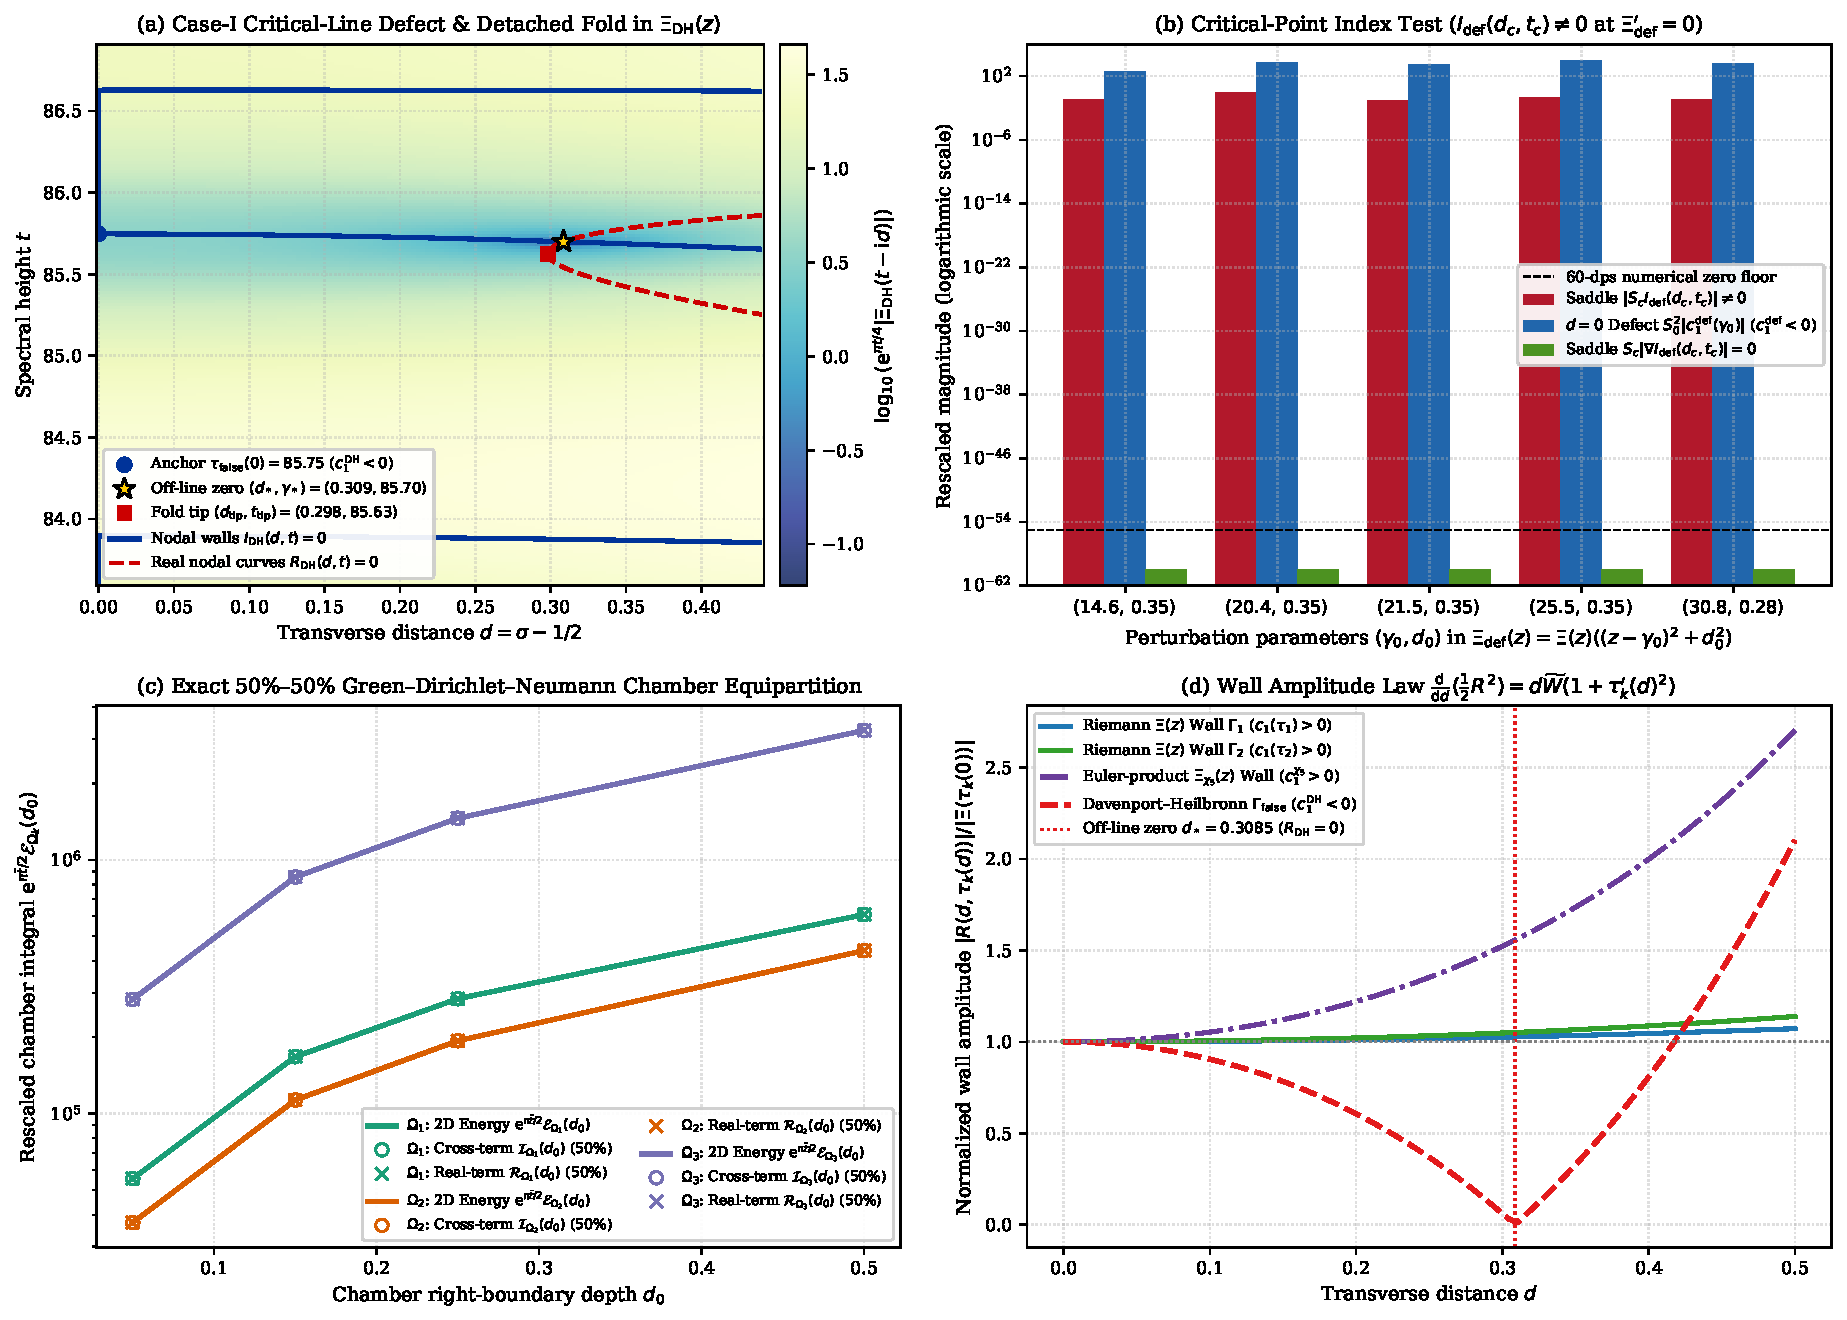
\includegraphics[width=0.98\textwidth]{figures/fig1_portal_frame_overdetermination_and_green_equipartition.pdf}
\caption{Nodal geometry and chamber flux equipartition (Sections~\ref{sec:macro}--\ref{sec:meso}): (a) Davenport--Heilbronn window $t \in [83.6,86.9]$, illustrating the Case-I branch $\Gamma_{\mathrm{false},1}$ from $\tau_{\mathrm{false},1}(0)=85.75$ ($c_1^{\DHf}<0$), the off-critical zero $(d_*,\gamma_*)=(0.3085,85.70)$ where $\Gamma_{\mathrm{false},1}$ crosses the detached real fold $R_{\DHf}=0$, and the fold vertex $(d_{\mathrm{tip}},t_{\mathrm{tip}})=(0.2981,85.63)$ where $W_{\DHf}=0$; (b) critical-point tests for $\Xi_{\defm}(z)=\Xi(z)((z-\gamma_0)^2+d_0^2)$ at interior roots $\Xi_{\defm}'(z_c)=0$, showing $I_{\defm}(d_c,t_c) \ne 0$ alongside the real-line defect $c_1^{\defm}(\gamma_0)<0$; (c) exact $50\%$--$50\%$ Green--Dirichlet--Neumann equipartition $\mathcal{I}_{\Omega_k}(d_0) \equiv \mathcal{R}_{\Omega_k}(d_0) \equiv \mathcal{E}_{\Omega_k}(d_0)$ across $\Omega_1,\Omega_2,\Omega_3$ of $\Xi(z)$; (d) branch amplitude evolution \eqref{eq:wall-amplitude-law} comparing $\Xi(z)$ and $\Xi_{\chi_5}(z)$ against $\Xi_{\DHf}(z)$.}
\label{fig:portal-macro-meso}
\end{figure}

\section{Weighted Prime-Simplex Dilogarithm Integrals: Factorized versus Additive Semiprime Weights}\label{sec:micro}

We now study a standalone analytical question in multiplicative number theory motivated by Dirichlet-polynomial truncations at the Riemann--Siegel horizon $N_\star(t) = \sqrt{t/(2\pi)}$ (with $L(t) := \ln(t/(2\pi)) = 2\ln N_\star(t)$). We emphasize upfront that the calculations in this section evaluate Prime-Number-Theorem simplex integrals and an elementary quadratic reference polynomial; as proved in Theorem~\ref{thm:additive-collapse} below, they do \emph{not} imply pointwise positivity $W(d,t) > 0$.

\subsection{Finite Dirichlet Sums, Toy Quadratic Polynomial, and Factorized Dilogarithm Integrals}\label{subsec:factorized-dilog}

For a finite prime cutoff $X = N_\star(t)^{2\theta}$ with $\theta \in (0,1/4)$ ($\tau := 2\theta = (\ln X)/\ln N_\star(t) \in (0,1/2)$) and $N = \lfloor N_\star(t) \rfloor$, the prime Dirichlet polynomial $\mathcal{P}_{>X}(s) := \sum_{X < p \le N} p^{-s}$ is an entire exponential sum whose algebraic square splits across the Dirichlet hyperbola $pq = N$:
\begin{equation}\label{eq:P-square-def}
\frac{1}{2}\mathcal{P}_{>X}(s)^2 = \mathcal{T}_{\le N}(s) + \mathcal{C}_{>N}(s), \qquad \mathcal{T}_{\le N}(s) := \frac{1}{2}\underset{pq \le N}{\sum_{X < p \le N}\,\sum_{X < q \le N}} (pq)^{-s}.
\end{equation}
If one replaces the truncated sum $1 + \mathcal{P}_{>X}(s) + \mathcal{T}_{\le N}(s)$ by a single complex variable $w = U + \ii V$ with a constant phenomenological multiplier $\eta \in (0,1]$ on $\frac{1}{2}w^2$, one obtains a toy quadratic polynomial whose algebraic root locus has a threshold at $\eta = 1/2$.

\begin{proposition}[Toy Quadratic Reference Polynomial]\label{prop:toy-quadratic}
For $\eta \in (0,1]$ and $w = U + \ii V \in \mathbb{C}$, set $\mathcal{Q}_\eta(U+\ii V) := 1 + (U+\ii V) + \frac{\eta}{2}(U+\ii V)^2$. Along the real axis $V=0$, $\mathcal{Q}_\eta(U) = 1 + U + \frac{\eta}{2}U^2$ has discriminant $\Delta(\eta) = 1 - 2\eta$: if $\eta > 1/2$, then $\Delta(\eta) < 0$ and
\begin{equation}\label{eq:spring-floor}
\bigl|\mathcal{Q}_\eta(U)\bigr|^2 = \Bigl[1 - \frac{1}{2\eta} + \frac{\eta}{2}\Bigl(U + \frac{1}{\eta}\Bigr)^2\Bigr]^2 \ge \Bigl(1 - \frac{1}{2\eta}\Bigr)^2 > 0 \qquad (\forall\,U \in \mathbb{R}),
\end{equation}
with complex zeros only at $U_0 = -1/\eta$, $V_0 = \pm\sqrt{2\eta-1}/\eta$; whereas if $\eta \le 1/2$, $\Delta(\eta) \ge 0$ and $\mathcal{Q}_\eta(U)$ vanishes on $\mathbb{R}$ at $U_\pm(\eta) = (-1 \pm \sqrt{1-2\eta})/\eta \le -2$.
\end{proposition}

\begin{proof}
Completing the square gives $1 + U + \frac{\eta}{2}U^2 = (1 - \frac{1}{2\eta}) + \frac{\eta}{2}(U + \frac{1}{\eta})^2$, which immediately yields \eqref{eq:spring-floor} for $\eta > 1/2$ and the real roots $U_\pm(\eta)$ for $\eta \le 1/2$. For $V \ne 0$, $\ImPt\,\mathcal{Q}_\eta(U+\ii V) = V(1 + \eta U) = 0$ forces $U = -1/\eta$, where $\RePt\,\mathcal{Q}_\eta(-1/\eta + \ii V) = 1 - \frac{1}{2\eta} - \frac{\eta}{2}V^2$.
\end{proof}

By Riemann--Stieltjes integration against Chebyshev's prime-counting function $\vartheta(x) = \sum_{p\le x}\ln p$ and the Prime Number Theorem $\vartheta(x) = x + O(x\exp(-c\sqrt{\ln x}))$ \cite{MontgomeryVaughan2007}, any smooth weight $g((\ln p)/\ln N_\star)$ satisfies $\sum_{X < p \le N_\star} \frac{g((\ln p)/\ln N_\star)}{p} = \int_\tau^1 \frac{g(u)}{u}\,\dd u + O(\|g\|_{W^{1,\infty}}(\ln X)^{-1})$, where $u = 2\alpha = (\ln p)/\ln N_\star \in [\tau,1]$. We first evaluate the exact polylogarithmic closed forms when a \emph{factorized} product weight $(1-u)^p(1-v)^p$ is integrated over the simplex $\Delta_\tau := \{(u,v) \in [\tau,1]^2 : u + v \le 1\}$.

\begin{theorem}[Closed-Form Euler Dilogarithm Laws for Factorized Simplex Weights]\label{thm:dilogarithm-laws}
For $\theta \in (0,1/4)$, $\tau := 2\theta \in (0,1/2)$, and $p \in \{0,1,2,3\}$, define the $1$D marginal integral $I_p(\theta) := \int_\theta^{1/2}\frac{(1-2\alpha)^p}{\alpha}\,\dd\alpha = \int_\tau^1 \frac{(1-u)^p}{u}\,\dd u$, the square integral $\mathcal{M}_{\sq}^{(p)}(\theta) := (I_p(\theta))^2$, and the factorized simplex integral
\begin{equation}\label{eq:M-tri-integral}
\mathcal{M}_{\tri,\facw}^{(p)}(\theta) := \underset{\alpha_1 + \alpha_2 \le 1/2}{\iint_{[\theta,1/2]^2}} \frac{(1-2\alpha_1)^p(1-2\alpha_2)^p}{\alpha_1\,\alpha_2}\,\dd\alpha_1\,\dd\alpha_2 = \iint_{\Delta_\tau} \frac{(1-u)^p(1-v)^p}{u\,v}\,\dd u\,\dd v,
\end{equation}
with ratio $\eta_{\facw}^{(p)}(\theta) := \mathcal{M}_{\tri,\facw}^{(p)}(\theta)/\mathcal{M}_{\sq}^{(p)}(\theta)$. Then
\begin{equation}\label{eq:Ip-closed}
\begin{aligned}
I_0(\theta) &= \ln\Bigl(\frac{1}{\tau}\Bigr), &\qquad I_1(\theta) &= \ln\Bigl(\frac{1}{\tau}\Bigr) - (1-\tau), \\
I_2(\theta) &= \ln\Bigl(\frac{1}{\tau}\Bigr) - \frac{1}{2}(1-\tau)(3-\tau), &\qquad I_3(\theta) &= \ln\Bigl(\frac{1}{\tau}\Bigr) - \frac{1}{3}(1-\tau)\bigl(2\tau^2 - 7\tau + 11\bigr),
\end{aligned}
\end{equation}
and the $2$D factorized simplex integrals $\mathcal{M}_{\tri,\facw}^{(p)}(\theta)$ are given in exact closed form by
\begin{align}
\mathcal{M}_{\tri}^{(0)}(\theta) &= \ln^2\tau + 2\,\Li_2(\tau) - \frac{\pi^2}{6}, \label{eq:M-tri-0} \\
\mathcal{M}_{\tri,\facw}^{(1)}(\theta) &= \mathcal{M}_{\tri}^{(0)}(\theta) - 2(1-\tau)\ln\Bigl(\frac{1-\tau}{\tau}\Bigr) + \Bigl(\frac{5}{2} - \tau\Bigr)(1-2\tau), \label{eq:M-tri-1} \\
\mathcal{M}_{\tri,\facw}^{(2)}(\theta) &= \mathcal{M}_{\tri}^{(0)}(\theta) - (1-\tau)(3-\tau)\ln\Bigl(\frac{1-\tau}{\tau}\Bigr) + \Bigl(\frac{31}{8} - \frac{13}{4}\tau + \tau^2\Bigr)(1-2\tau), \label{eq:M-tri-2} \\
\mathcal{M}_{\tri,\facw}^{(3)}(\theta) &= \mathcal{M}_{\tri}^{(0)}(\theta) - \frac{1}{3}(1-\tau)\bigl(11 - 7\tau + 2\tau^2\bigr)\ln\Bigl(\frac{1-\tau}{\tau}\Bigr) \nonumber\\
&\quad + \Bigl(\frac{1801}{360} - \frac{1199}{180}\tau + \frac{218}{45}\tau^2 - \frac{89}{45}\tau^3 + \frac{49}{90}\tau^4 - \frac{1}{9}\tau^5\Bigr)(1-2\tau). \label{eq:M-tri-3}
\end{align}
At $\theta = 1/6$ ($\tau = 1/3$), the factorized ratios are $\eta^{(0)}(1/6) = 0.2439550996 < 1/2$, $\eta_{\facw}^{(1)}(1/6) = 0.4955987356 < 1/2$, $\eta_{\facw}^{(2)}(1/6) = 0.6768906167 > 2/3 > 1/2$ (with $50\%$ root $\theta_{*,50\%}^{(2)} = 0.1905498467 > \frac{1}{2\ee} = 0.1839397206 > \frac{1}{6}$), and $\eta_{\facw}^{(3)}(1/6) = 0.7980906218 > 3/4$ ($\theta_{*,50\%}^{(3)} = 0.2039297718$).
\end{theorem}

\begin{proof}
Expanding $(1-u)^p$ binomially on $[\tau,1]$ gives \eqref{eq:Ip-closed}. For $p=0$, $\mathcal{M}_{\tri}^{(0)}(\theta) = \int_\tau^{1-\tau} \frac{\ln(1-u) - \ln\tau}{u}\,\dd u = [-\Li_2(1-\tau) + \Li_2(\tau)] - (\ln\tau)[\ln(1-\tau) - \ln\tau]$; substituting Euler's reflection identity $\Li_2(1-\tau) = \frac{\pi^2}{6} - \Li_2(\tau) - (\ln\tau)\ln(1-\tau)$ \cite{Lewin1981} cancels the mixed term $-(\ln\tau)\ln(1-\tau)$ identically and yields \eqref{eq:M-tri-0}. The complete derivations of \eqref{eq:M-tri-1}--\eqref{eq:M-tri-3} are given in Appendix~\ref{app:dilogarithm}.
\end{proof}

\subsection{True Additive Semiprime Wronskian Weight Collapse and Hyperbola Duality}\label{subsec:additive-and-duality}

Crucially, in the truncated Riemann--Siegel / Wronskian approximation $\widehat{W}(d,t)$ at height $t$, an individual composite mode $n = pq \le N_\star(t)$ does \emph{not} carry the factorized product weight $\omega_p(t)^2\omega_q(t)^2 = (\ln N_\star)^4(1-u)^2(1-v)^2$; rather, as a single Dirichlet term $(pq)^{-s}$, its stationary-phase frequency distance to the horizon $N_\star(t)$ is \emph{additive} in $\ln p$ and $\ln q$:
\begin{equation}\label{eq:true-additive-weight}
\omega_{pq}(t) := \ln\Bigl(\frac{N_\star(t)}{pq}\Bigr) = \ln N_\star(t) - \ln p - \ln q = (\ln N_\star(t))(1 - u - v).
\end{equation}
Our next theorem evaluates the exact closed form of the true additive semiprime simplex integral and proves that at $\theta = 1/6$ it falls \emph{strictly below} $1/2$---and even below the unweighted ratio $\eta^{(0)}(1/6)$.

\begin{theorem}[True Additive Semiprime Weight Closed Forms and Collapse Below $1/2$]\label{thm:additive-collapse}
For $\theta \in (0,1/4)$, $\tau := 2\theta \in (0,1/2)$, and $p \in \{1,2\}$, define the additive semiprime simplex integral
\begin{equation}\label{eq:M-tri-add-def}
\mathcal{M}_{\tri,\addw}^{(p)}(\theta) := \iint_{\Delta_\tau} \frac{(1 - u - v)^p}{u\,v}\,\dd u\,\dd v, \qquad \eta_{\addw}^{(p)}(\theta) := \frac{\mathcal{M}_{\tri,\addw}^{(p)}(\theta)}{\mathcal{M}_{\sq}^{(p)}(\theta)}.
\end{equation}
Then $\mathcal{M}_{\tri,\addw}^{(1)}(\theta)$ and $\mathcal{M}_{\tri,\addw}^{(2)}(\theta)$ satisfy the exact closed-form identities
\begin{align}
\mathcal{M}_{\tri,\addw}^{(1)}(\theta) &= \mathcal{M}_{\tri}^{(0)}(\theta) - 2(1-\tau)\ln\Bigl(\frac{1-\tau}{\tau}\Bigr) + 2(1-2\tau), \label{eq:M-tri-add-1} \\
\mathcal{M}_{\tri,\addw}^{(2)}(\theta) &= \mathcal{M}_{\tri}^{(0)}(\theta) - (1-\tau)(3-\tau)\ln\Bigl(\frac{1-\tau}{\tau}\Bigr) + \Bigl(\frac{7}{2} - 2\tau\Bigr)(1-2\tau), \label{eq:M-tri-add-2}
\end{align}
with strictly positive polynomial deficits relative to the factorized integrals \eqref{eq:M-tri-1}--\eqref{eq:M-tri-2} for all $\tau \in (0,1/2)$:
\begin{equation}\label{eq:fac-minus-add}
\mathcal{M}_{\tri,\facw}^{(1)}(\theta) - \mathcal{M}_{\tri,\addw}^{(1)}(\theta) = \frac{1}{2}(1-2\tau)^2 > 0, \qquad \mathcal{M}_{\tri,\facw}^{(2)}(\theta) - \mathcal{M}_{\tri,\addw}^{(2)}(\theta) = \frac{1}{8}(1-2\tau)^2(3 - 4\tau) > 0.
\end{equation}
In particular, at $\theta = 1/6$ ($\tau = 1/3$), $\mathcal{M}_{\tri,\addw}^{(2)}(1/6) = 0.006624144034$ versus $\mathcal{M}_{\tri,\facw}^{(2)}(1/6) = 0.029772292182$ (deficit $\frac{5}{216} = 0.023148148148$), and the normalized capture ratios collapse strictly below $1/2$:
\begin{equation}\label{eq:eta-add-collapse}
\eta_{\addw}^{(1)}(1/6) = 0.1978366884 < \frac{1}{2}, \qquad \eta_{\addw}^{(2)}(1/6) = 0.1506038202 < \eta^{(0)}(1/6) = 0.2439550996 < \frac{1}{2}.
\end{equation}
\end{theorem}

\begin{proof}
On $\Delta_\tau$, we have the algebraic identities $(1-u)(1-v) - (1-u-v) = uv$ and
\[
(1-u)^2(1-v)^2 - (1-u-v)^2 = (1 - u - v + uv)^2 - (1 - u - v)^2 = uv\bigl[2(1 - u - v) + uv\bigr].
\]
Dividing both identities by $uv$ cancels the denominator $uv$ identically and leaves pure polynomials on the right triangle $\Delta_\tau = \{(u,v) : u \ge \tau,\, v \ge \tau,\, u+v \le 1\}$ of leg length $\ell := 1 - 2\tau > 0$:
\[
\mathcal{M}_{\tri,\facw}^{(1)}(\theta) - \mathcal{M}_{\tri,\addw}^{(1)}(\theta) = \iint_{\Delta_\tau} 1\,\dd u\,\dd v = \frac{1}{2}\ell^2 = \frac{1}{2}(1-2\tau)^2,
\]
and setting $x = u - \tau$, $y = v - \tau$ ($x,y \ge 0$, $x+y \le \ell$) gives $\iint_{\Delta_\tau} 2(\ell - x - y)\,\dd x\,\dd y = \frac{1}{3}\ell^3$ and $\iint_{\Delta_\tau} (\tau+x)(\tau+y)\,\dd x\,\dd y = \frac{1}{2}\tau^2\ell^2 + \frac{1}{3}\tau\ell^3 + \frac{1}{24}\ell^4 = \frac{1}{24}\ell^2(1 + 4\tau)$ since $\ell = 1 - 2\tau$. Summing gives $\frac{1}{3}\ell^3 + \frac{1}{24}\ell^2(1+4\tau) = \frac{1}{24}\ell^2[8(1-2\tau) + 1 + 4\tau] = \frac{1}{8}(1-2\tau)^2(3-4\tau) > 0$ for all $\tau \in (0,1/2)$, proving \eqref{eq:fac-minus-add}. Subtracting \eqref{eq:fac-minus-add} from \eqref{eq:M-tri-1}--\eqref{eq:M-tri-2} establishes \eqref{eq:M-tri-add-1}--\eqref{eq:M-tri-add-2}, and evaluating at $\tau = 1/3$ yields \eqref{eq:eta-add-collapse}.
\end{proof}

Finally, we record the exact reflection identity for the individual prime weights $\omega_p(t)$ and $\omega_q(t)$ across the Dirichlet hyperbola $pq = N_\star(t)$.

\begin{theorem}[Dirichlet Hyperbola Reflection Duality and Fourth-Order Apex Pinching]\label{thm:hyperbola-duality}
Let $t > 2\pi$ and $N_\star(t) = \sqrt{t/(2\pi)}$. For $(p,q) \in (X,N_\star]^2$, set $\omega_p(t) := \ln(N_\star(t)/p)$, $\omega_q(t) := \ln(N_\star(t)/q)$, $\omega_{pq}(t) := \ln(N_\star(t)/(pq))$, and $m_{\dual}(pq) := N_\star(t)^2/(pq) = t/(2\pi pq)$. Then:
\begin{enumerate}[label=\upshape(\alph*),leftmargin=2.2em]
\item $(p,q)$ lies in the forward triangle $pq \le N_\star(t)$ iff $\omega_{pq}(t) \ge 0$, and in the reflected corner $pq > N_\star(t)$ iff $\omega_{pq}(t) < 0$ ($m_{\dual}(pq) \in [1, N_\star(t))$).
\item The individual prime weights satisfy $\omega_p(t) + \omega_q(t) \equiv \ln(N_\star(t)^2/(pq)) \equiv \ln m_{\dual}(pq) = L(t)[1 - (\alpha_1+\alpha_2)]$.
\item By the Arithmetic--Geometric Mean inequality on $\omega_p(t),\omega_q(t) \ge 0$, the factorized product weight pinches to fourth order at the apex $pq \to N_\star(t)^2$ ($m_{\dual}(pq) \to 1^+$):
\begin{equation}\label{eq:apex-pinching}
0 \le \bigl(\omega_p(t)\,\omega_q(t)\bigr)^2 \le \frac{1}{16}\bigl(\omega_p(t) + \omega_q(t)\bigr)^4 = \frac{1}{16}\bigl(\ln m_{\dual}(pq)\bigr)^4 \longrightarrow 0.
\end{equation}
\end{enumerate}
\end{theorem}

\begin{proof}
Part~(a) is immediate from $\omega_{pq}(t) = \ln(N_\star(t)/(pq))$. Adding $\omega_p(t) = \ln N_\star - \ln p$ and $\omega_q(t) = \ln N_\star - \ln q$ gives $\ln(N_\star^2/(pq)) = \ln m_{\dual}(pq)$, proving (b), and squaring $\omega_p\omega_q \le \frac{1}{4}(\omega_p+\omega_q)^2$ yields \eqref{eq:apex-pinching}.
\end{proof}

\begin{table}[htbp]
\centering
\caption{Sixty-five-decimal certification of Section~\ref{sec:micro}: (Part~A) closed-form Euler dilogarithm $\Li_2(2\theta)$ factorized capture fractions $\eta_{\facw}^{(p)}(\theta)$ ($p=0,1,2,3$) contrasted with the true additive semiprime Wronskian ratio $\eta_{\addw}^{(2)}(\theta)$; (Part~B) discrete prime-sum convergence $\eta_{\mathrm{disc}}^{(p)}(N_\star)$ to the continuous factorized $\Li_2(1/3)$ limits at $\theta=1/6$ up to $N_\star = 10^5$ ($9578$ primes); (Part~C) Dirichlet hyperbola reflection duality $\omega_p+\omega_q \equiv \ln m_{\dual}(pq)$ and fourth-order apex pinching at $t = 10^8$ ($N_\star = 3989.4228$).}
\label{tab:micro-certification}
\tiny
\setlength{\tabcolsep}{1.0pt}
\renewcommand{\arraystretch}{1.14}
\begin{tabular}{@{}cccccccc@{}}
\toprule
\multicolumn{8}{c}{\textbf{Part A: Factorized $\eta_{\facw}^{(p)}(\theta)$ vs.\ Additive Semiprime $\eta_{\addw}^{(2)}(\theta)$ Dilogarithm Ratios Across $\theta \in [0.05, 0.24]$}} \\
\midrule
Benchmark & $\theta$ & $\eta^{(0)}(\theta)$ & $\eta_{\facw}^{(1)}(\theta)$ & $\eta_{\facw}^{(2)}(\theta)$ & $\eta_{\addw}^{(2)}(\theta)$ & Floor $(1-\frac{1}{2\eta_{\facw}^{(2)}})^2$ & $\eta_{\facw}^{(3)}(\theta)$ \\
\midrule
Deep cutoff & $0.05000000$ & $0.72845562$ & $0.92880886$ & $0.98017181$ & $0.77116356$ & $+0.23998780$ & $0.99428000$ \\
$p=0$ $\theta_{*,50\%}^{(0)}$ & $0.10669705$ & $\mathbf{0.50000000}$ & $0.78533491$ & $0.90957454$ & $0.47157787$ & $+0.20276348$ & $0.96225919$ \\
$p=2$ $\theta_{*,75\%}^{(2)}$ & $0.15361739$ & $0.29963060$ & $0.57313128$ & $\mathbf{0.75000000}$ & $0.21246691$ & $+0.11111111$ & $0.85701362$ \\
\textbf{Cubic $1/6$} & $\mathbf{0.16666667}$ & $\mathbf{0.24395510}$ & $\mathbf{0.49559874}$ & $\mathbf{0.67689062}$ & $\mathbf{0.15060382}$ & $\mathbf{+0.06829172}$ & $\mathbf{0.79809062}$ \\
Mertens $1/(2\ee)$ & $0.18393972$ & $0.17257503$ & $0.38129980$ & $0.55478859$ & $0.08263747$ & $+0.00975309$ & $0.68732436$ \\
$p=2$ $\theta_{*,50\%}^{(2)}$ & $0.19054985$ & $0.14649770$ & $0.33471880$ & $\mathbf{0.50000000}$ & $0.06175914$ & $0.00000000$ & $0.63294631$ \\
Fifth-root $1/5$ & $0.20000000$ & $0.11103091$ & $0.26651789$ & $0.41426365$ & $0.03741656$ & Real roots & $0.54227319$ \\
$p=3$ $\theta_{*,50\%}^{(3)}$ & $0.20392977$ & $0.09707058$ & $0.23796348$ & $0.37632744$ & $0.02925292$ & Real roots & $\mathbf{0.50000000}$ \\
Quarter $0.24$ & $0.24000000$ & $0.00610514$ & $0.01844521$ & $0.03495745$ & $0.00014442$ & Real roots & $0.05476574$ \\
\midrule
\multicolumn{8}{c}{\textbf{Part B: Discrete Prime-Sum Convergence $\eta_{\mathrm{disc}}^{(p)}(N_\star)$ to Continuous Factorized $\mathrm{Li}_2(1/3)$ Laws at $\theta = 1/6$}} \\
\midrule
$N_\star = \lfloor\sqrt{t/(2\pi)}\rfloor$ & $X$ & Primes $M$ & $\eta_{\mathrm{disc}}^{(0)}(N_\star)$ & $\eta_{\mathrm{disc}}^{(1)}(N_\star)$ & $\eta_{\mathrm{disc}}^{(2)}(N_\star)$ & $\frac{\eta_{\mathrm{disc}}^{(2)}}{1-\eta_{\mathrm{disc}}^{(2)}}$ & $\eta_{\mathrm{disc}}^{(3)}(N_\star)$ \\
\midrule
$398$ ($t = 10^6$) & $7$ & $74$ & $0.147826$ & $0.345842$ & $0.518747$ & $1.077909$ & $0.654850$ \\
$1261$ ($t = 10^7$) & $10$ & $201$ & $0.264895$ & $0.535458$ & $0.720307$ & $2.575352$ & $0.836156$ \\
$3989$ ($t = 10^8$) & $15$ & $544$ & $0.232742$ & $0.486772$ & $0.672969$ & $2.057814$ & $0.797661$ \\
$12615$ ($t = 10^9$) & $23$ & $1498$ & $0.200526$ & $0.433336$ & $0.615770$ & $1.602607$ & $0.746482$ \\
$39894$ ($t = 10^{10}$) & $34$ & $4184$ & $0.229646$ & $0.478319$ & $0.662165$ & $1.960025$ & $0.787100$ \\
$10^5$ ($6.3\cdot 10^{10}$) & $46$ & $9578$ & $0.232219$ & $0.481580$ & $0.665147$ & $1.986388$ & $0.789519$ \\
\textbf{$\mathrm{Li}_2(1/3)$ Limit} & $1/6$ & $\infty$ & $\mathbf{0.243955}$ & $\mathbf{0.495599}$ & $\mathbf{0.676891}$ & $\mathbf{2.094927}$ & $\mathbf{0.798091}$ \\
\midrule
\multicolumn{8}{c}{\textbf{Part C: Dirichlet Hyperbola Reflection Duality and Fourth-Order Apex Pinching at $t = 10^8$ ($N_\star = 3989.4228$)}} \\
\midrule
Pair $(p,q)$ & $pq$ & $\omega_{pq}(t)/2$ & $m_{\dual}(pq)$ & $|\omega_p+\omega_q-\ln m_{\dual}|$ & $(\frac{\omega_p\omega_q}{(\ln N_\star)^2})^2$ & $\frac{16(\omega_p\omega_q)^2}{(\ln m_{\dual})^4}$ & Sector \\
\midrule
$(17, 19)$ & $323 \le N_\star$ & $+1.25687$ & $49273.98$ & $< 10^{-65}$ & $1.8022 \times 10^{-1}$ & $0.999788 \le 1$ & Forward $\mathcal{T}_{\le N}$ \\
$(41, 89)$ & $3649 \le N_\star$ & $+0.04460$ & $4361.60$ & $< 10^{-65}$ & $6.4122 \times 10^{-2}$ & $0.982967 \le 1$ & Forward $\mathcal{T}_{\le N}$ \\
$(61, 67)$ & $4087 > N_\star$ & $-0.01208$ & $3894.18$ & $< 10^{-65}$ & $6.1759 \times 10^{-2}$ & $0.999742 \le 1$ & Reflected $\mathcal{C}_{>N}$ \\
$(503, 701)$ & $352603 > N_\star$ & $-2.24085$ & $45.14$ & $4.75 \times 10^{-66}$ & $2.7436 \times 10^{-3}$ & $0.984876 \le 1$ & Reflected $\mathcal{C}_{>N}$ \\
$(3967, 3989)$ & $15824363$ & $-4.14283$ & $1.0058 \to 1$ & $2.20 \times 10^{-66}$ & $7.5509 \times 10^{-17}$ & $0.005251 \le 1$ & Apex ($4$th-ord.\ $0$) \\
\bottomrule
\end{tabular}
\end{table}

\begin{figure}[htbp]
\centering
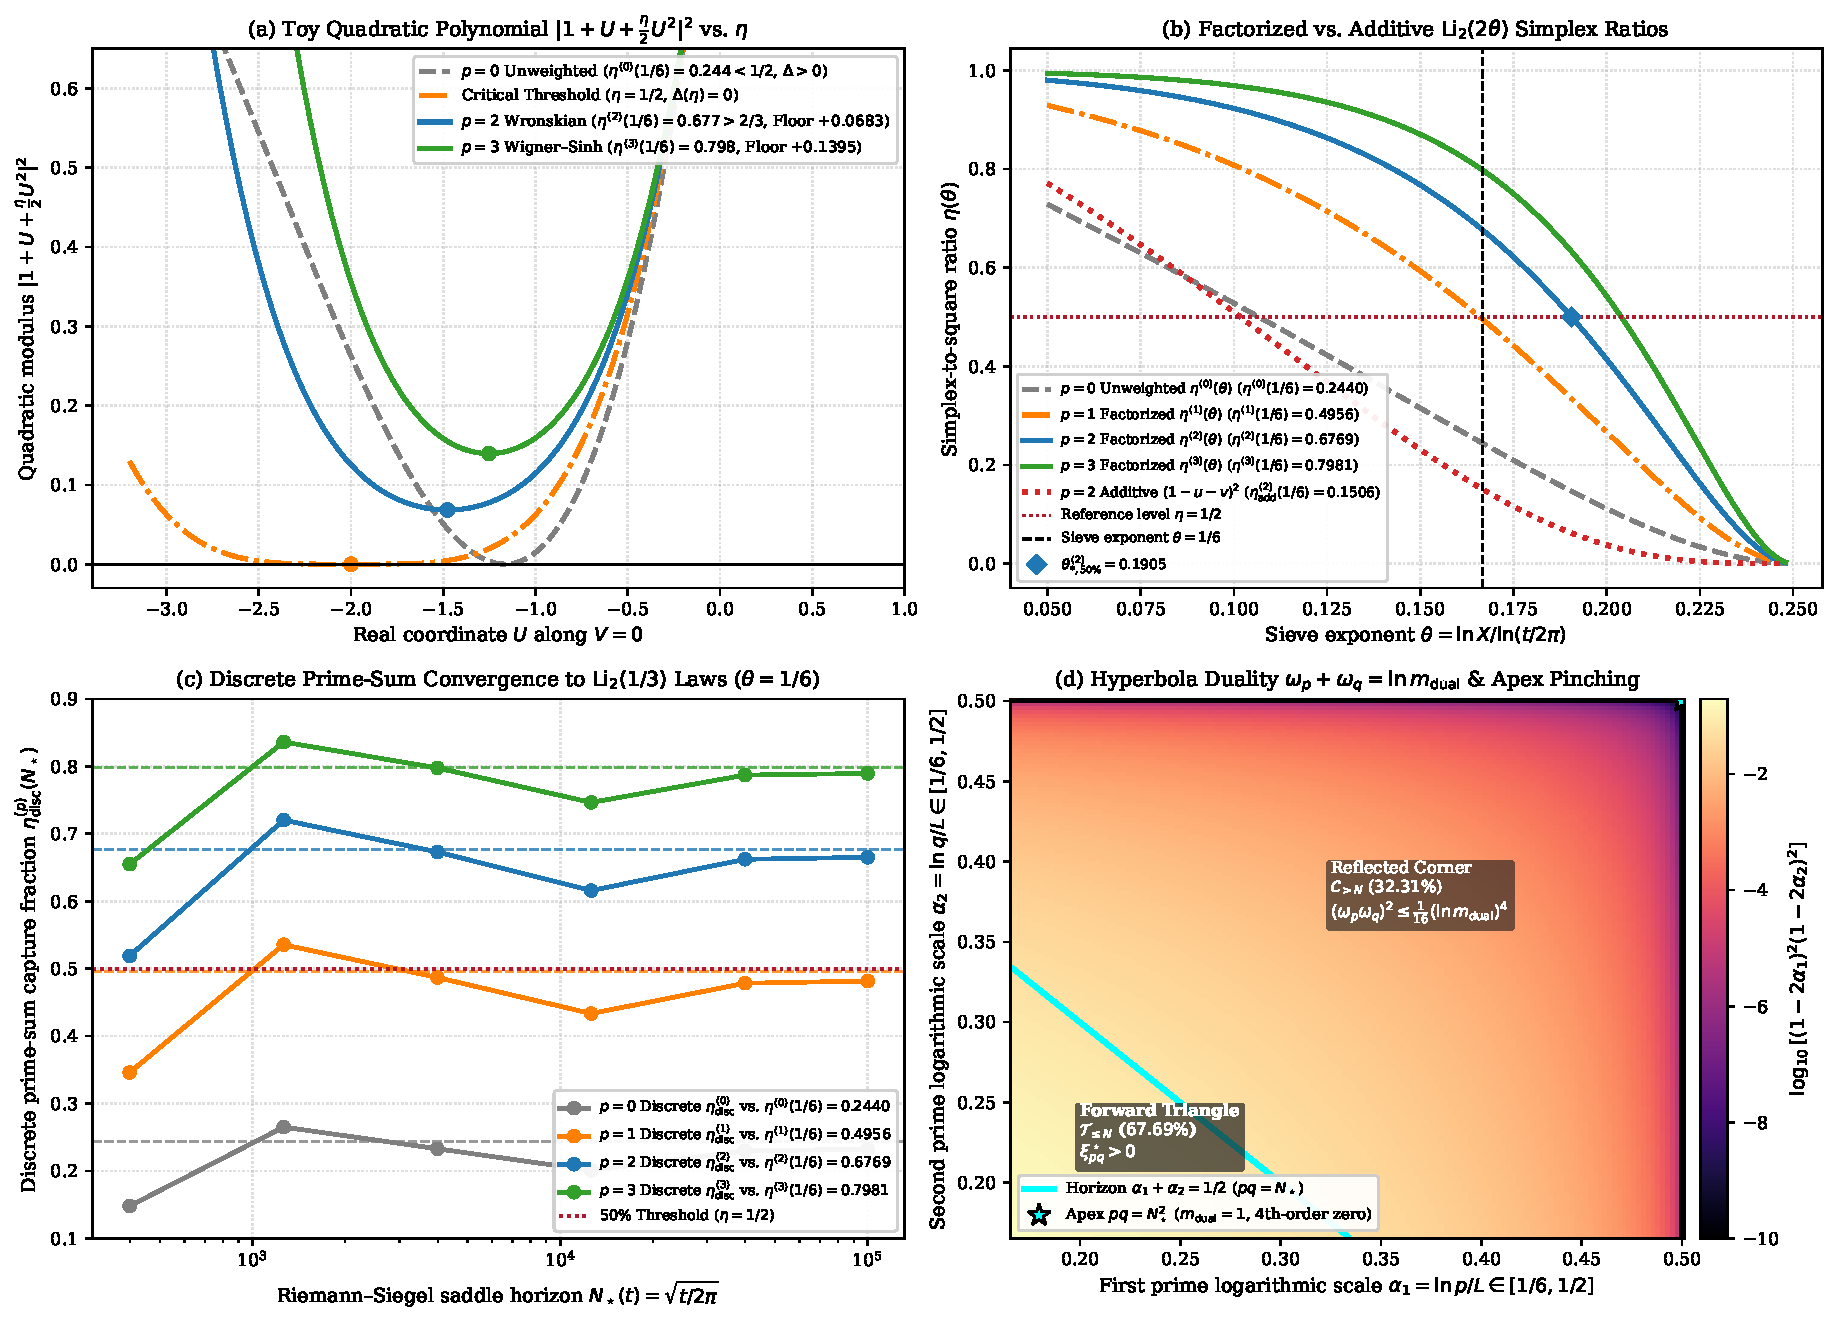
\includegraphics[width=0.98\textwidth]{figures/fig2_dilogarithm_horizon_damping_and_hyperbola_duality.pdf}
\caption{Weighted prime-simplex dilogarithm integrals and hyperbola duality (Section~\ref{sec:micro}): (a) toy reference polynomial $|1 + U + \frac{\eta}{2}U^2|^2$ vs.\ $\eta$; (b) closed-form Euler dilogarithm ratios comparing factorized weights $\eta_{\facw}^{(p)}(\theta)$ ($p=0,1,2,3$) against the true additive semiprime weight $\eta_{\addw}^{(2)}(\theta)$ ($\eta_{\addw}^{(2)}(1/6)=0.1506 < 1/2$); (c) discrete prime-sum convergence $\eta_{\mathrm{disc}}^{(p)}(N_\star)$ to $\eta_{\facw}^{(p)}(1/6)$ up to $N_\star = 10^5$; (d) Dirichlet hyperbola reflection duality $\omega_p+\omega_q = \ln m_{\dual}(pq)$ and fourth-order apex pinching across $[\frac{1}{6},\frac{1}{2}]^2$.}
\label{fig:micro-dilogarithm}
\end{figure}

\section{Scope, Limitations, and Open Questions}\label{sec:scope}

To maintain complete mathematical clarity \cite{Bombieri2000,Edwards1974,Titchmarsh1986}, we separate the unconditional identities proved in this paper from their structural limitations:
\begin{enumerate}[label=\upshape(\arabic*),leftmargin=2.2em]
\item \textbf{Unconditional Harmonic and Polylogarithmic Identities:} Theorems~\ref{thm:nodal-dichotomy} (local Cauchy--Riemann nodal monotonicity, bounded loop/arch exclusion, and curvature conservation), \ref{thm:green-equipartition} ($50\%$--$50\%$ Green--Dirichlet--Neumann chamber equipartition \eqref{eq:boxed-green-equipartition}), \ref{thm:wronskian-slope-reciprocity} (Wronskian--slope reciprocity and fold-tip vanishing), \ref{thm:dilogarithm-laws} (factorized $\Li_2(2\theta)$ formulas), \ref{thm:additive-collapse} (additive semiprime $\Li_2(2\theta)$ formulas and $\eta_{\addw}^{(2)}(1/6)=0.150604<1/2$), and \ref{thm:hyperbola-duality} (hyperbola reflection duality) are unconditional analytical theorems, verified to $52$--$65$ decimal places.
\item \textbf{Global Nodal Topology and Critical-Point Difficulty:} As detailed in Remarks~\ref{rem:codim3-fallacy}--\ref{rem:hairpin-caveat} and Theorem~\ref{thm:index-and-dh}(b), naive codimension-three counting fails in $1$-parameter families such as de Bruijn--Newman heat flow and proves nothing for a fixed function; unbounded hairpin components of $\{I=0\}$ require global Phragm\'{e}n--Lindel\"{o}f and Euler-product arguments as $d \to +\infty$; and ruling out interior critical points $\Xi'(t-\ii d)=0$ in $d>0$ (Case~II in the Craven--Csordas--Smith / Ki--Kim index formula \cite{CravenCsordasSmith1987,KiKim2000}) is comparable in difficulty to the Riemann Hypothesis itself \cite{Speiser1934}. Furthermore, the chamber equipartition $\mathcal{W}_{\Omega_k}(d_0) = 2\mathcal{E}_{\Omega_k}(d_0) > 0$ is an \emph{integrated} positivity law across $[\tau_k(d_0),\tau_{k+1}(d_0)]$ (which holds even on the split subchambers $\Omega_{\DHf,\mathrm{L}}$ and $\Omega_{\DHf,\mathrm{R}}$ of $\Xi_{\DHf}$ in Table~\ref{tab:meso-certification}B) and does not imply pointwise positivity $W(d_0,t) > 0$.
\item \textbf{No Mean-Field Link from Simplex Dilogarithm Integrals to Pointwise $W(d,t) > 0$:} Theorem~\ref{thm:additive-collapse} shows that once the ad-hoc factorized weight $(1-u)^2(1-v)^2$ is replaced by the true additive stationary-phase weight $(1-u-v)^2$ of a semiprime $n = pq \le N_\star(t)$, the simplex-to-square ratio drops from $0.676891$ to $0.150604 < 1/2$. In addition, oscillatory phases $p^{-\ii t} = \ee^{-\ii t\ln p}$ and the divergence of infinite prime Dirichlet series inside $0 < \sigma < 1$ prevent any rigorous reduction of pointwise $W(d,t)$ to the toy polynomial $\mathcal{Q}_\eta(U)$ of Proposition~\ref{prop:toy-quadratic}. Establishing unconditional lower bounds on $c_1(t)$ or $Z_{\mathbb{C}}(\Xi')$ remains open.
\end{enumerate}

\appendix

\section{Exact Polylogarithmic Derivations of the Simplex Integrals}\label{app:dilogarithm}

Set $u = 2\alpha_1$, $v = 2\alpha_2$, and $\tau = 2\theta \in (0,1/2)$, so $\Delta_\tau = \{(u,v) \in [\tau,1]^2 : u+v \le 1\}$ fibers over $u \in [\tau, 1-\tau]$ with $v \in [\tau, 1-u]$. Write $f_p(v) := (1-v)^p/v = \frac{1}{v} - P_p(v)$, where $P_0(v)=0$, $P_1(v)=1$, $P_2(v)=2-v$, and $P_3(v)=3-3v+v^2$, with antiderivatives $Q_p(y) := \int_0^y P_p(v)\,\dd v$:
\[
Q_0(y) = 0, \qquad Q_1(y) = y, \qquad Q_2(y) = 2y - \frac{1}{2}y^2, \qquad Q_3(y) = 3y - \frac{3}{2}y^2 + \frac{1}{3}y^3.
\]
Since $\int_\tau^{1-u} f_p(v)\,\dd v = \ln(\frac{1-u}{\tau}) - [Q_p(1-u) - Q_p(\tau)]$, substituting $f_p(u) = \frac{1}{u} - P_p(u)$ into $\mathcal{M}_{\tri,\facw}^{(p)}(\theta) = \int_\tau^{1-\tau} f_p(u)(\int_\tau^{1-u} f_p(v)\,\dd v)\,\dd u$ decomposes $\mathcal{M}_{\tri,\facw}^{(p)}(\theta)$ into three pieces:
\begin{align}
\mathcal{M}_{\tri,\facw}^{(p)}(\theta) &= \int_{\tau}^{1-\tau} \frac{1}{u}\ln\Bigl(\frac{1-u}{\tau}\Bigr)\,\dd u - \int_{\tau}^{1-\tau} \Bigl[P_p(u)\ln\Bigl(\frac{1-u}{\tau}\Bigr) + \frac{Q_p(1-u) - Q_p(\tau)}{u}\Bigr]\,\dd u \nonumber\\
&\quad + \int_{\tau}^{1-\tau} P_p(u)\,\bigl[Q_p(1-u) - Q_p(\tau)\bigr]\,\dd u. \label{eq:app-three-pieces}
\end{align}

\paragraph{\textbf{Piece 1: The Dilogarithmic Core $\mathcal{M}_{\tri}^{(0)}(\theta)$.}}
Since $-\int_0^x \frac{\ln(1-u)}{u}\,\dd u = \Li_2(x)$, the first integral in \eqref{eq:app-three-pieces} equals
\[
\mathcal{M}_{\tri}^{(0)}(\theta) = \bigl[-\Li_2(1-\tau) + \Li_2(\tau)\bigr] - (\ln\tau)\bigl[\ln(1-\tau) - \ln\tau\bigr].
\]
Substituting Euler's reflection identity $-\Li_2(1-\tau) = -\frac{\pi^2}{6} + \Li_2(\tau) + (\ln\tau)\ln(1-\tau)$ \cite{Lewin1981} cancels $+(\ln\tau)\ln(1-\tau)$ against $-(\ln\tau)\ln(1-\tau)$ and gives $\mathcal{M}_{\tri}^{(0)}(\theta) = \ln^2\tau + 2\,\Li_2(\tau) - \frac{\pi^2}{6}$, proving \eqref{eq:M-tri-0}.

\paragraph{\textbf{Piece 2: Harmonic Polynomial Reduction of the Logarithmic Terms.}}
Writing $P_p(v) = \sum_{k=1}^p (1-v)^{k-1}$, we have $Q_p(1) - Q_p(1-u) = \sum_{k=1}^p \frac{u^k}{k}$ and $R_p(u) := \frac{Q_p(1)-Q_p(1-u)}{u} = \sum_{k=1}^p \frac{u^{k-1}}{k}$. Using $Q_p(1-u)-Q_p(\tau) = [Q_p(1)-Q_p(\tau)] - u R_p(u)$ and integrating $P_p(u)\ln(\frac{1-u}{\tau}) = \frac{\dd}{\dd u}[Q_p(u)-Q_p(1)]\ln(\frac{1-u}{\tau})$ by parts over $[\tau,1-\tau]$ (noting $\int_\tau^{1-\tau} R_p(1-u)\,\dd u = \int_\tau^{1-\tau} R_p(u)\,\dd u$) gives
\begin{equation}\label{eq:piece2-exact}
\begin{aligned}
-\int_{\tau}^{1-\tau} \Bigl[P_p(u)\ln\Bigl(\frac{1-u}{\tau}\Bigr) &+ \frac{Q_p(1-u) - Q_p(\tau)}{u}\Bigr]\,\dd u \\
&= -2\bigl[Q_p(1)-Q_p(\tau)\bigr]\ln\Bigl(\frac{1-\tau}{\tau}\Bigr) + 2\int_{\tau}^{1-\tau} R_p(u)\,\dd u,
\end{aligned}
\end{equation}
where $2[Q_1(1)-Q_1(\tau)] = 2(1-\tau)$, $2[Q_2(1)-Q_2(\tau)] = (1-\tau)(3-\tau)$, and $2[Q_3(1)-Q_3(\tau)] = \frac{1}{3}(1-\tau)(11 - 7\tau + 2\tau^2)$.

\paragraph{\textbf{Piece 3: Exact Polynomial Terms.}}
Adding $2\int_\tau^{1-\tau} R_p(u)\,\dd u$ from \eqref{eq:piece2-exact} to the third integral $\int_\tau^{1-\tau} P_p(u)[Q_p(1-u)-Q_p(\tau)]\,\dd u > 0$ in \eqref{eq:app-three-pieces} over $[\tau,1-\tau]$ gives:
\begin{itemize}[leftmargin=1.8em]
\item For $p=1$: $2\int_\tau^{1-\tau} 1\,\dd u + \int_\tau^{1-\tau} (1-u-\tau)\,\dd u = 2(1-2\tau) + \frac{1}{2}(1-2\tau)^2 = (\frac{5}{2} - \tau)(1-2\tau)$, proving \eqref{eq:M-tri-1}.
\item For $p=2$: $2\int_\tau^{1-\tau}(1+\frac{u}{2})\,\dd u = \frac{5}{2}(1-2\tau)$, while $\int_\tau^{1-\tau}(2-u)[2(1-u-\tau) - \frac{1}{2}((1-u)^2-\tau^2)]\,\dd u = (\frac{11}{8} - \frac{13}{4}\tau + \tau^2)(1-2\tau)$; adding the two gives $(\frac{31}{8} - \frac{13}{4}\tau + \tau^2)(1-2\tau)$, proving \eqref{eq:M-tri-2}.
\item For $p=3$: $2\int_\tau^{1-\tau}(1+\frac{u}{2}+\frac{u^2}{3})\,\dd u + \int_\tau^{1-\tau}(3-3u+u^2)[Q_3(1-u)-Q_3(\tau)]\,\dd u = (\frac{1801}{360} - \frac{1199}{180}\tau + \frac{218}{45}\tau^2 - \frac{89}{45}\tau^3 + \frac{49}{90}\tau^4 - \frac{1}{9}\tau^5)(1-2\tau)$, proving \eqref{eq:M-tri-3}.
\end{itemize}

\section*{Use of AI and computational verification}

In accordance with academic publishing transparency standards, the author discloses that Google Gemini was used to assist in formatting the AMS-\LaTeX{} manuscript, symbolically cross-checking the polylogarithmic antiderivatives in Appendix~\ref{app:dilogarithm}, and executing the $65$-decimal-place arbitrary-precision \texttt{mpmath} and $35$-decimal-place rigorous interval arithmetic (\texttt{mpmath.iv}) verification suite (\url{scripts/verify_paper14_portal_dilogarithm_synthesis.py}). All mathematical definitions, theorem statements, analytical proofs, scope limitations, and numerical benchmarks were independently verified by the author; every assertion in the verification suite exits with code \texttt{0}.

\begin{thebibliography}{99}

\bibitem{Bombieri2000}
E.~Bombieri, \emph{Problems of the Millennium: The Riemann Hypothesis}, Clay Mathematics Institute, Cambridge, MA, 2000.

\bibitem{BombieriGhosh2011}
E.~Bombieri and A.~Ghosh, \emph{Around the Davenport--Heilbronn function}, Uspekhi Mat.\ Nauk \textbf{66} (2011), no.~2, 15--66; Russian Math.\ Surveys \textbf{66} (2011), no.~2, 221--270.

\bibitem{CravenCsordasSmith1987}
T.~Craven, G.~Csordas, and W.~Smith, \emph{The zeros of derivatives of entire functions and the P\'{o}lya--Wiman conjecture}, Ann.\ of Math.\ (2) \textbf{125} (1987), no.~2, 405--431.

\bibitem{CsordasNorfolkVarga1986}
G.~Csordas, T.~S.~Norfolk, and R.~S.~Varga, \emph{The Riemann hypothesis and the Tur\'{a}n inequalities}, Trans.\ Amer.\ Math.\ Soc.\ \textbf{296} (1986), no.~2, 521--541.

\bibitem{DavenportHeilbronn1936}
H.~Davenport and H.~Heilbronn, \emph{On the zeros of certain Dirichlet series I, II}, J.\ London Math.\ Soc.\ \textbf{11} (1936), 181--185, 307--312.

\bibitem{Edwards1974}
H.~M.~Edwards, \emph{Riemann's Zeta Function}, Academic Press, New York, 1974.

\bibitem{Hecke1937}
E.~Hecke, \emph{\"{U}ber die Bestimmung Dirichletscher Reihen durch ihre Funktionalgleichung}, Math.\ Ann.\ \textbf{112} (1936), 664--699.

\bibitem{Jensen1913}
J.~L.~W.~V.~Jensen, \emph{Recherches sur la th\'{e}orie des \'{e}quations}, Acta Math.\ \textbf{36} (1913), 181--195.

\bibitem{KiKim2000}
H.~Ki and Y.-O.~Kim, \emph{On the number of nonreal zeros of real entire functions and the Fourier--P\'{o}lya conjecture}, Duke Math.\ J.\ \textbf{104} (2000), no.~1, 45--73.

\bibitem{Laguerre1898}
E.~Laguerre, \emph{\OE uvres de Laguerre}, Tome I, Gauthier-Villars, Paris, 1898.

\bibitem{Lewin1981}
L.~Lewin, \emph{Polylogarithms and Associated Functions}, North-Holland Publishing Co., New York--Amsterdam, 1981.

\bibitem{MontgomeryVaughan2007}
H.~L.~Montgomery and R.~C.~Vaughan, \emph{Multiplicative Number Theory I. Classical Theory}, Cambridge Studies in Advanced Mathematics, vol.~97, Cambridge Univ.\ Press, Cambridge, 2007.

\bibitem{Newman1976}
C.~M.~Newman, \emph{Fourier transforms with only real zeros}, Proc.\ Amer.\ Math.\ Soc.\ \textbf{61} (1976), no.~2, 245--251.

\bibitem{Polya1926}
G.~P\'{o}lya, \emph{Bemerkung \"{u}ber die Integraldarstellung der Riemannschen $\xi$-Funktion}, Acta Math.\ \textbf{48} (1926), 305--317.

\bibitem{Riemann1859}
B.~Riemann, \emph{\"{U}ber die Anzahl der Primzahlen unter einer gegebenen Gr\"{o}sse}, Monatsber.\ K\"{o}nigl.\ Preuss.\ Akad.\ Wiss.\ Berlin (1859), 671--680.

\bibitem{RodgersTao2020}
B.~Rodgers and T.~Tao, \emph{The De Bruijn--Newman constant is non-negative}, Forum Math.\ Pi \textbf{8} (2020), e6, 62~pp.

\bibitem{Speiser1934}
A.~Speiser, \emph{Geometrisches zur Riemannschen Zetafunktion}, Math.\ Ann.\ \textbf{110} (1934), 514--521.

\bibitem{Titchmarsh1986}
E.~C.~Titchmarsh, \emph{The Theory of the Riemann Zeta-Function}, 2nd ed., edited and with a preface by D.~R.~Heath-Brown, Clarendon Press, Oxford, 1986.

\bibitem{Wigner1932}
E.~Wigner, \emph{On the quantum correction for thermodynamic equilibrium}, Phys.\ Rev.\ \textbf{40} (1932), 749--759.

\end{thebibliography}

\end{document}
